%\documentclass[aps,prd,nofootinbib,amsmath,notitlepage]{revtex4-1}
\documentclass[11pt]{article}
\usepackage{jcappub}
\usepackage{amssymb,esvect,amsmath,graphicx,latexsym,amsthm,slashed,eso-pic,fullpage}
\usepackage[final]{pdfpages}
\usepackage{array}
\usepackage{soul}
\usepackage[normalem]{ulem}
\usepackage{multirow}
\usepackage{pbox}
\DeclareMathOperator{\ev}{eV} \DeclareMathOperator{\kev}{KeV} \DeclareMathOperator{\mev}{MeV} \DeclareMathOperator{\gev}{GeV} \DeclareMathOperator{\tev}{TeV} \DeclareMathOperator{\cm}{cm} \DeclareMathOperator{\barn}{barn} \DeclareMathOperator{\g}{g} \DeclareMathOperator{\km}{km} \DeclareMathOperator{\pb}{pb} \DeclareMathOperator{\s}{s} \DeclareMathOperator{\yr}{yr}\DeclareMathOperator{\gyr}{Gyr} \DeclareMathOperator{\kg}{kg} \DeclareMathOperator{\mpc}{Mpc} \DeclareMathOperator{\few}{few} \DeclareMathOperator{\kel}{K}
\newcommand{\cA}{{\cal A}} \newcommand{\cC}{{\cal C}} \newcommand{\cD}{{\cal D}} \newcommand{\cE}{{\cal E}} \newcommand{\cF}{{ \cal F}} \newcommand{\cH}{{\cal H}} \newcommand{\cJ}{{\cal J}} \newcommand{\cL}{{\cal L}} \newcommand{\cM}{{\cal M}} \newcommand{\cN}{{\cal N}} \newcommand{\cO}{{\cal O}} \newcommand{\cP}{{ \cal P}} \newcommand{\tp}{{ \tilde p}} \newcommand{\cR}{{\cal R}} \newcommand{\cS}{{\cal S}}
\newcommand{\ep}{\epsilon} \newcommand{\vp}{\varphi} \newcommand{\half}{\frac12}
\newcommand{\ie}{{\it i.e.~}}  \newcommand{\eg}{{\it e.g.~}}
\newcommand{\pt}{\partial} \def\d{{\rm d}}  \def\oL{\overline} \def\wh{\widehat}
\newcommand{\pL}{\left(} \newcommand{\pR}{\right)} \newcommand{\bL}{\left[} \newcommand{\bR}{\right]} \newcommand{\cbL}{\left\{} \newcommand{\cbR}{\right\}} \newcommand{\mL}{\left|} \newcommand{\mR}{\right|} \newcommand{\ER}{E_R}
\newcommand{\beq}{\begin{equation}} \newcommand{\eeq}{\end{equation}}
\newcommand{\bea}{\begin{eqnarray}} \newcommand{\eea}{\end{eqnarray}}
\newcommand{\alg}[1]{\begin{align} \begin{split} #1 \end{split}  \end{align}}
\newcommand{\vev}[1]{\langle {#1} \rangle}
\newcommand{\tenx}[1]{\times 10^{#1}}
\newcommand{\Eq}[1]{Eq.~(\ref{#1})} \newcommand{\Eqs}[2]{Eqs.~(\ref{#1}) and (\ref{#2})} \newcommand{\Eqm}[2]{Eqs.~(\ref{#1}) through (\ref{#2})}
\newcommand{\Sec}[1]{Sec.~\ref{#1}} \newcommand{\Secs}[2]{Secs.~\ref{#1} and \ref{#2}} \newcommand{\Secm}[2]{Secs.~\ref{#1} through \ref{#2}}
\newcommand{\Fig}[1]{Fig.~\ref{#1}} \newcommand{\Figs}[2]{Figs.~\ref{#1} and \ref{#2}}
\newcommand{\Tab}[1]{Tab.~\ref{#1}}
\newcommand{\App}[1]{App.~\ref{#1}}
\DeclareMathOperator{\br}{Br} \DeclareMathOperator{\tr}{Tr}
\newcommand{\arxiv}[1]{{\href{http://arxiv.org/abs/#1}{\tt #1}}}

\newcommand{\sdm}[1]{\textcolor{blue}{\textbf{(#1 -- SDM)}}}

\newcommand{\sjwColor}{red}
\newcommand{\sjw}[1]{{\color{\sjwColor} #1}}
\newcommand{\sjwrm}[1]{{\color{\sjwColor}\protect\sout{#1}}}
\newcommand{\sjwrp}[2]{\sjwrm{#1} \sjw{#2}}
\newcommand{\sjwtt}[1]{{\color{\sjwColor}\tt #1}} 


\newcommand{\vgColor}{magenta}
\newcommand{\vg}[1]{{\color{\vgColor} #1}}

\begin{document}
\title{Prospects for Distinguishing Dark Matter Models Using Annual Modulation}
\author[a,b]{Samuel J.~Witte,}
\author[c]{Vera Gluscevic,}
\author[d]{and Samuel D.~McDermott}


\affiliation[a]{University of California, Los Angeles, Department of Physics and Astronomy, Los Angeles, CA 90095}

\affiliation[b]{Fermi National Accelerator Laboratory, Center for Particle
Astrophysics, Batavia, IL 60510}

\affiliation[c]{School of Natural Sciences, Institute for Advanced Study, Einstein Drive, Princeton NJ 08540, USA}

\affiliation[d]{C.~N.~Yang Institute for Theoretical Physics, Stony Brook, NY, USA}\subheader{\rm YITP-SB-16-NN}

\abstract{


}

\maketitle

\section{Introduction} \setcounter{page}{2}

A vast array of independent astrophysical and cosmological observations testifyes to the existence of a non-baryonic form of matter in the universe. This so-called dark matter (DM) is the dominant source of the gravitational potential wells that dictate the dynamics and structure of the universe, but dark matter particles have yet to be observed in a laboratory setting. Despite an experimental direct detection program that has now been mature for several decades, all evidence in favor of the existence of dark matter still comes from its gravitational interactions with baryons \cite{Bauer:2013ihz}.

As the next--generation direct detection experiments that incorporate increasingly sensitive detection technologies come online, they will start to probe the final portions of DM parameter space before encountering the irreducible neutrino backgrounds \sjwtt{Add citations. Projections for future DD.} \cite{Cushman:2013zza,Billard:2013qya,Ruppin:2014bra,Davis:2014ama,Dent:2016iht}. Generation 2 (G2) experiments that are currently taking data \cite{} may well be on the cusp of important discoveries, as many interesting theories of DM predict scattering cross sections that live in these portions of paramters space. For example, heavy $SU(2)$--doublet and --triplet fermions, such as the Higgsinos and the wino of supersymmetry, are expected to have cross sections of order $\sigma_{\rm SI} \sim \cO(\few\tenx{-48})\cm^2$ (just about an order of magnitude below the current limits \cite{}), fixed by their Standard Model gauge quantum numbers alone \cite{Hill:2011be,Hill:2013hoa,Hill:2014yxa}, while a heavy $SU(2)$-singlet fermion, like the bino, is around an order of magnitude lower depending on its coannihilation partner \cite{Berlin:2015njh}. Models with kinematically suppressed tree--level scattering may also be embedded in more complete dark sectors that have loop--level cross sections in this same range \cite{Ipek:2014gua,McDermott:2014rqa,Appelquist:2015yfa,Appelquist:2015zfa}.

Because so many theories can be accommodated in the parameter space that will be imminently probed by a variety of experiments, it is timely to plan for the science opportunities associated with the first detection of DM particles. Most notably, in case of a confirmed detection, understanding the high--energy dark sector dynamics will solely rely on examining low--energy recoils of detector elements and solving the ``inverse problem'' to identify the right underlying description of DM--baryon interactions from the experimental measurements. On the other hand, all the information about the dark sector interactions accessible to these measurements is contained within the coefficients of the ``effective field theory of dark matter direct detection'' \cite{Fitzpatrick:2012ix, Anand:2013yka}. This effective description also captures the nontrivial nuclear physics induced by some of the best--motivated UV--complete theories of dark matter \cite{Gresham:2014vja, Gluscevic:2015sqa} through an exhaustable list of nuclear responses. It thus provides a systematic framework for calssifying and describing a wide variety of DM interaction theories, and we will utilize it in this work. 
 
However, due to Poisson noise and degeneracies in the shape of the recoil spectra amongst different interactions, DM model selection, and distinguishing amongst different effective descriptions has been shown to present a difficult task in practice, for a single target material. Recent studies have shown that discriminating between interactions is possible only for strong signals (with hundreds of observed recoil events), and only when measurements on targets with sufficiently diverse nuclear physics characteristics are jointly analyzed \cite{}. Thus, using energy spectra to break degeneracies in the dark matter modeling space crucially relies on ``complementary'' nuclear physics characteristics of available target materials \cite{McDermott:2011hx,Peter:2013aha,Gluscevic:2014vga,Catena:2014epa,Catena:2014hla,Dent:2015zpa,Gluscevic:2015sqa,Ruppin:2014bra}, but even so does not guarantee successful model selection \cite{Gluscevic:2014vga}.

On the other hand, almost since the dawn of direct--detection--related DM studies, the motion of the Earth relative to DM bound in the galactic halo has been predicted to provide a distinctive DM signature \cite{Freese:1987wu, Freese:2012xd,Lee:2013xxa,Britto:2014wga,DelNobile:2015nua,Kouvaris:2015xga} through characteristic annual modulation of the expected event rate of nuclear recoils. Recent work \cite{DelNobile:2015tza,DelNobile:2015rmp} pointed out that non--standard interaction cross sections containing a non--factorizable velocity dependence could produce a modulation signal that is unique to each target element. More generally, a non--trivial velocity dependence in the cross section effectively changes the velocity integral that governs the total event rate in any given experiment, and produces a characteristic modulation signal. It may thus be expected that interaction models that differ solely by the power of velocity of their corresponding cross sections may differ by the phase and/or amplityde of the annual modulation signal they display. 

Motivated by this argument, here we propose that analysis of time dependence of scattering events can help discriminate between interaction models whose recoil energy spectra are otherwise degenerate on a single target material. Using the method of \cite{}, we evaluate the ehancement in prospects for accurate model selection when the annual modulation signal is analysed in combination with recoil--energy measurements in the next--generation direct detection experiments. 


%Almost since the dawn of the study of direct detection experiments, the annual modulation of the rate \cite{Freese:1987wu} arising from the motion of Earth relative to dark matter bound in the galactic halo has been appreciated to provide a distinctive dark matter signature, as have its higher harmonics (see e.g. \cite{Freese:2012xd,Lee:2013xxa,Britto:2014wga,DelNobile:2015nua,Kouvaris:2015xga}). \sjw{Earth's velocity with respect to the dark matter `wind' is at a maximum around June $1^{\rm st}$ and a minimum around December $1^{\rm st}$. For a fixed low energy threshold experiment, conventional wisdom would suggest that increasing the relative velocity between Earth and the dark matter `wind' should enhance the number of dark matter particles which can produce an observable recoil above threshold, and thus the of maximum of the scattering rate should occur around June $1^{\rm st}$. While this is true at large energies, standard differential cross sections (\ie those satisfying $d\sigma/d\ER \propto v^{-2}$) actually produce a phase flip, such that at low energies the rate is maximized in December. This feature occurs because the differential cross section is enhanced by low velocity scattering. }

%The aforementioned arguments, however, only hold for conventional virialized velocity distributions and standard differential cross sections. The disturbance of phase space from dark matter substructure \cite{Green:2000ga,Gelmini:2000dm,DelNobile:2015nua} and the gravitational influence of the solar system \cite{Lee:2013wza,DelNobile:2015nua} have been shown to a non-negligible impact on the annual modulation, in particular modifying the phase of the modulation. Additionally, it was recently pointed out in~\cite{DelNobile:2015tza,DelNobile:2015rmp} that differential cross sections with higher order dark matter velocity dependence produce a phase at low energies that is roughly $5$ months out of phase with conventionally considered interactions. Furthermore, \cite{DelNobile:2015tza,DelNobile:2015rmp} emphasized that differential cross sections containing a non-factorizable velocity and target dependence can produce a modulation that is unique to each target element. A proper analysis of direct detection data including the time information of nuclear recoils may therefore have the potential to elucidate unique astrophysical processes and atypical dark matter-nuclei interactions. \sjwtt{Note to self, add more citations to the above section}  

%Since the local distribution of dark matter is at this moment poorly understood, we will focus in this work on quantitatively understanding the extent to which including information on the modulation of the rate can enhance the ability of future direct detection experiments to correctly differentiate dark matter-nuclei interactions with approximately degenerate recoil spectrum but distinct time behavior. Interestingly, we find that the additional discrimination power from timing information will allow some of the most popular detector designs to go beyond detection and significantly improve model identification, even for models with approximately degenerate recoil spectra.  This is possible because, as previously mentioned, additional factors of $v^2$ appearing in the differential cross section alters the phase of the modulation. 






In \Sec{sec:dd} we review the calculation of the direct detection scattering rate. \Sec{sec:eft} introduces the concept of dark matter effective field theory, discusses how momentum and velocity dependent cross sections can result in nonstandard scattering, and reviews dark matter models which have nearly degenerate recoil spectra but distinguishing time dependence. We introduce our analysis procedure in \Sec{sec:procedure} and present our results in \Sec{sec:results}. We conclude in \Sec{sec:conclusion}.


  

\section{Scattering in Direct Detection Experiments}\label{sec:dd}

\subsection{Basics}

The key measurement of most direct detection experiments is the nuclear recoil energy spectrum---the number count of nuclear recoil events per recoil energy $E_R$, per unit time $t$, per unit target mass,
\begin{equation}
\frac{dR}{dE_R dt}(E_R,t) =  \frac{\rho_\chi}{m_T m_\chi} \int\limits_{v_{\mathrm{min}}}^{v_{\mathrm{esc, lab}}}  v f(\mathrm{\mbox{\bf{v}}},t) \frac{d\sigma_T}{dE_R} (E_R,v) d^3v ,
\label{eq:dRdEr_general}
\end{equation}
where $\rho_\chi$ is the local DM density; $m_\chi$ is the DM particle mass; $m_T$ is the mass of the target nucleus $T$; $\mathrm{\mbox{\bf{v}}}$ is DM velocity vector of magnitude $v$ (in the lab frame); $f(\mathrm{\mbox{\bf{v}}}, t)$ is the observed DM velocity distribution; $d\sigma_T/dE_R=m_T \sigma_T /2\mu_T^2 v^2$ is the differential cross section for DM scattering off a nucleus $T$; and $\mu_T\equiv\frac{m_Tm_\chi}{m_T+m_\chi}$ is the reduced mass of the DM particle and the target nucleus. Integration limits are the minimum velocity od a DM particle needed to produce a nuclear recoil of energy $E_R$, which, for elastic scattering reads $v_\mathrm{min} = \sqrt{m_T E_R/2\mu_T^2}$, and the escape velocity from the Galactic halo in the lab frame, $v_{\mathrm{esc, lab}}$.

The differential rate in \Eq{eq:dRdEr_general} is determined by the experimental setup, the DM astrophysical and particle properties, the nuclear properties of the target material, and the DM--nucleus interaction.\footnote{Throughout this paper we use $T$ to denote the nuclear target and $N$ to denote a nucleon, either neutron $n$ or proton $p$} For the purposes of this study, we set the astrophysical parameters to the following values \cite{Bovy:2013raa,Piffl:2013mla}: $\rho_\chi=0.3$ GeV/cm$^3$; $v_{\mathrm{esc}} = 533$ km/sec (in the Galactic frame), and assume that $f(\mathrm{\mbox{\bf{v}}})$ is a Maxwellian distribution in the Galactic frame, with a rms speed of $155$ km/sec and a mean speed equal to the Sun's rotational velocity around the Galactic center, $v_\textrm{lag}=220$ km/sec.

The underlying particle physics interaction model determines the calculation of the recoil rate through the differential scattering cross section ${d\sigma_T}/{dE_R}$ \cite{Gluscevic:2015sqa,Gresham:2014vja}. This quantity has a normalization (in units of cm${}^2$) which is a free parameter of the model. Different interactions display different functional dependences on $E_R$ and $v$, as discussed in detail in Refs.~\cite{Gluscevic:2015sqa,Gresham:2014vja} and summarized below in \S\ref{subsec:momentum_velocity}.

The total rate $R$ of nuclear recoil events (per unit time and unit mass) is given by the integral of the differential rate within the nuclear--recoil energy window $\cE$ of a given experiment\footnote{For simplicity, we assume unit efficiency of detection within the analysis window, and rescale individual experimetal exposures to take this assumption into account when choosing experimental parameters to represent the capabilities of G2 experiments.}, $R(t)=\int_\cE \frac{dR}{dE_R dt} dE_R$. In turn, the total expected number of events $\langle N_\mathrm{tot}\rangle$ for a fiducial target mass $\cM_\textrm{fid}$, in experiment that started observation at a time $t_1$ and ended at a time $t_2$, within energy window $\cE$ is
\beq
\langle N_\mathrm{tot}\rangle =  \cM_\textrm{fid} \int\limits_{t_1}^{t_2} \int\limits_\cE  \frac{dR}{dE_R dt}(E_R,t)\,dE_R \,dt.
\eeq

\subsection{Momentum and Velocity Dependendence}
\label{subsec:momentum_velocity}

Traditional focus on the two standard scattering cases: spin--independent (SI) and spin--dependent (SD) scattering (where the former involves coherent contributions from the entire nucleus and the cross section scales quadratically with nucleon number, and the latter scales with the total nuclear spin) obscures the richness of phenomenologies accessible to direct detection experiments, which can arise when the two standard interactions are suppressed for various reasons \cite{}. Here we summarize the effective field theory that catalogues all possible energy and velocity dependencies of the cross section, and thus delineates the modeling space for interactions probed by these experiments in most general terms. In the \S\ref{sec:models}, we highlight several well--motivated examples of interesting scattering models which we use in this work to examine the extent to which including time information can enhance identification of the underlying model.

%The target nucleus in direct detection experiments is chosen to have large principal quantum numbers according to which the experiment is categorized as spin--independent (SI) or spin-dependent. Spin-independent scattering involves coherent contributions from the entire nucleus, such that the cross section scales quadratically with nucleon number. This is to be contrasted with the spin-dependent rate which scales with the total nuclear spin, a quantity that is typically concentrated in a single nucleon. Thus, experiments are usually based on elements selected for having large $A$ or large total spin, with the former experiments dubbed ``spin-independent'' and exhibiting reach to smaller absolute values of the overall cross section. \sjwtt{Guys... I'm gonna want to come back and address this paragraph. I understand the gist and I'm not vehemently opposed to having something like this, but the wording as it just doesn't seem correct.} 

%Such simplistic classification obscures the fact that this dichotomy strictly refers to the dependence on nuclear spin, and does not necessarily imply a hierarchy of expected rates. Many responses sensitive to a diversity of nuclear ``charges'' and ``currents'' can be classified as ``spin-independent'' \cite{Fitzpatrick:2012ix}, most of which are suppressed by small kinematic factors. Suppression of spin-independent scattering can lead to novel signatures in direct detection experiments. Consistently counting the pertinent small factors, and thus acquiring intuition for what might be seen in future experiments, requires a proper effective field theory expansion. 


%The function $\frac{d\sigma_T}{dE_R} (E_R,v)$ in \Eq{eq:dRdEr_general} contains the interesting particle physics of the DM--nucleus scattering and determines the energy and time dependence of the observable recoil event rate. 
The effective field theory of DM direct detection \cite{Fitzpatrick:2012ix, Anand:2013yka} relies on an expansion in two small kinematic variables: $|\vec q|/m_N$, where $\vec q$ is the change in momentum of the DM particle during the scattering, and $|\vec v_\perp|$ is the orthogonal component of the relative velocity of the initial--state particles. For an incoming (outgoing) DM three--momentum $\vec p(\vec p')$, incoming (outgoing) nuclear three--momentum $\vec k$ $(\vec k')$, and a reduced mass $\mu_{\chi N} \equiv m_\chi m_N/(m_\chi +m_N)$, these factors are $\vec q=\vec p'-\vec p=\vec k-\vec k'$, and $\vec v_\perp=\frac{\vec p}{m_\chi}-\frac{\vec k}{m_N}+\frac{\vec q}{2\mu_{\chi N}}$, respectively.
The momentum transfer is directly related to the nuclear recoil energy as $\vec{q}^{\, 2} =2m_TE_R$. 

These expansion parameters are of the same order of magnitude, but it is important to note that they manifest differently in the observables of the scattering events. In particular, terms \vg{(changed ``responses'' to terms, is this ok?)} that enter at higher order in $|\vec q|/m_N$ deliver a vanishing event rate at both small and large momentum transfer (or recoil--energy), with a maximum rate at some intermediate recoil energy, producing a ``turnover feature'' in the recoil--energy spectrum (see .... in Fig.~\ref{}, for example). \vg{What about light-mediator cases? There is a second type of spectral signature we are not mentioning, like in the case of millicharge...} On the other hand, higher--order terms in $| \vec v_\perp|$ produce rates that monotonically decrease with energy, quantitatively similar to the standard SI or SD interaction case (see .... in Fig.~\ref{}, for example). 

As was demonstrated by Ref.~\cite{Gluscevic:2015sqa}, the interaction models that feature different momentum dependence can be differentiated from each other using a single nuclear target, provided a sufficiently large exposure and event number counts; however, the latter class of models---those that differ only by the power of velocity dependence---are far more difficult to disentangle, leaving substantial degeneracy between well--motivated interaction models. In the following, we develop an intuition for how this degeneracy might be overcome, using annual modulation and time dependence of the scattering rate.

\subsection{Time Dependendence}
\label{subsec:time}

In \Eq{eq:dRdEr_general}, the differential rate of nuclear recoils is explicitly denoted as depending on time, which arises as a consequence of the Earth's harmonic motion around the Sun. This ``annual modulation'' of the DM particle ``wind'', as observed in the lab frame, is additionally affected by ``gravitational focusing'' of DM particles in the Sun's potential well \cite{Danby01021957,Griest:1987vc,Sikivie:2002bj,Alenazi:2006wu}. Overall, these effects are expected to give rise to an energy--dependent modulation of the total nuclear recoil rate in direct detection experiments. 

\begin{figure*}
\centering
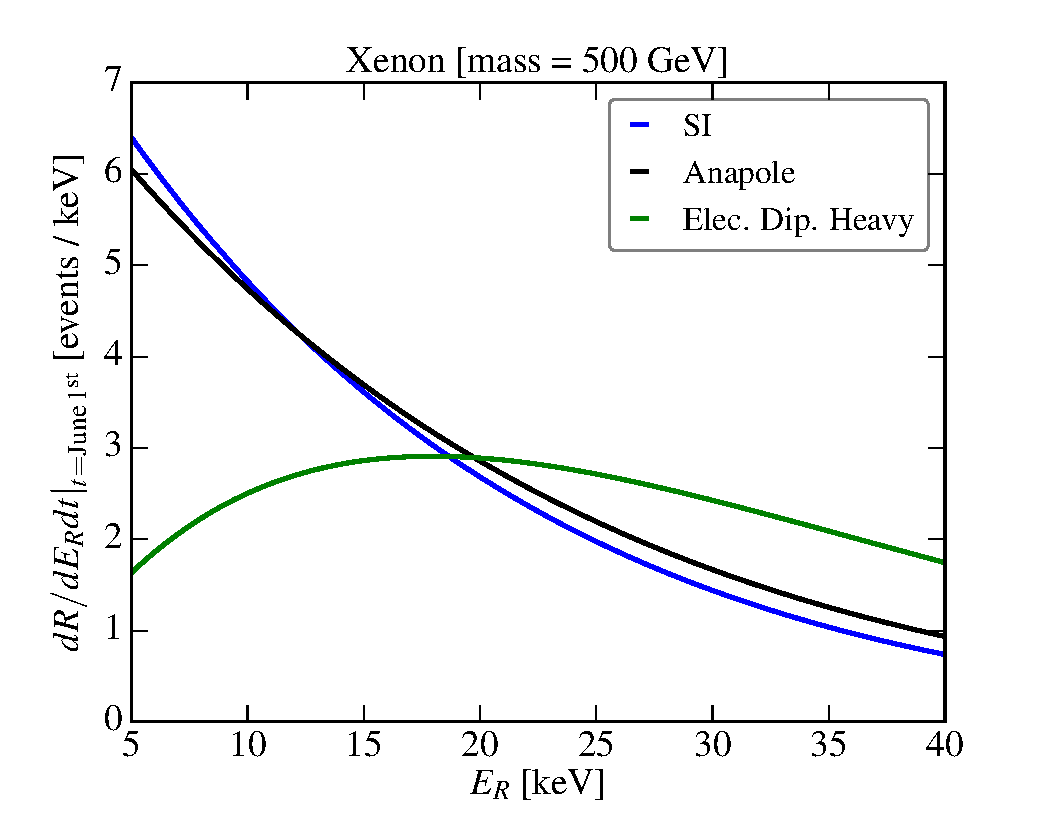
\includegraphics[width=0.49\textwidth, trim=0.cm 0.0cm 0.cm 0.0cm,clip=true]{plots/RecoilComparison_500GeV.pdf}
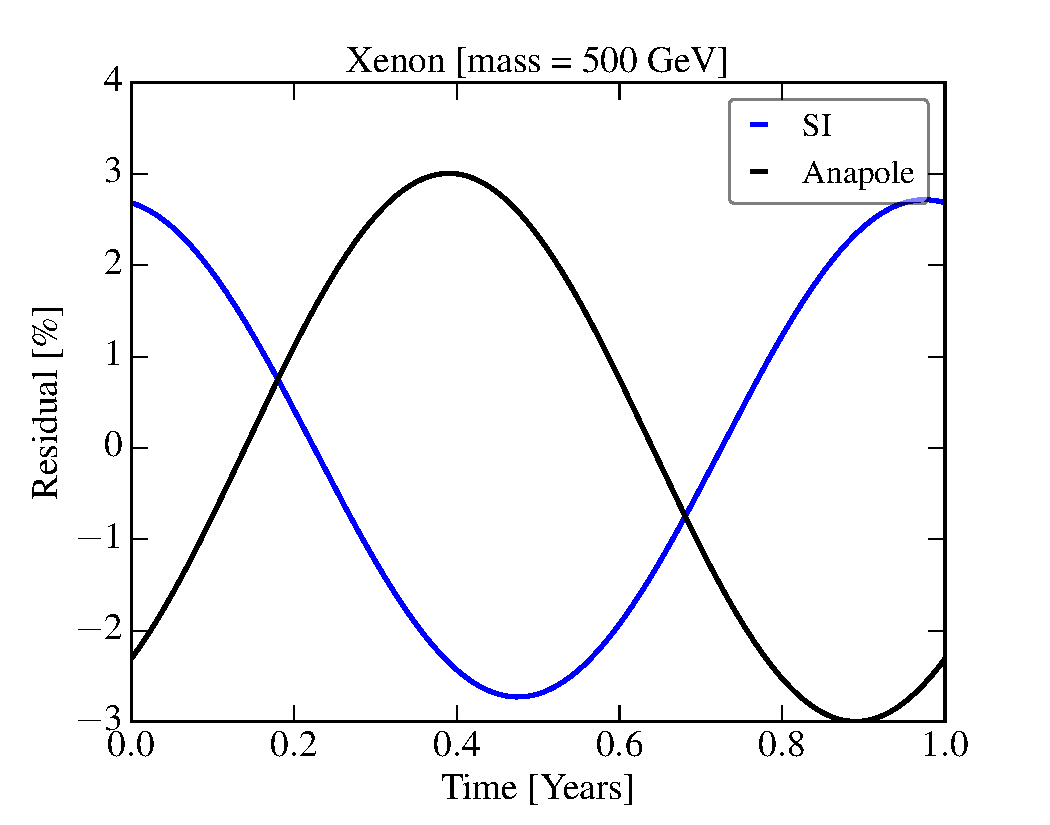
\includegraphics[width=0.49\textwidth, trim=0.cm 0.0cm 0.cm 0.0cm,clip=true]{plots/Xenon_SIvsAnapole_500GeV_Residual_Theory.pdf}
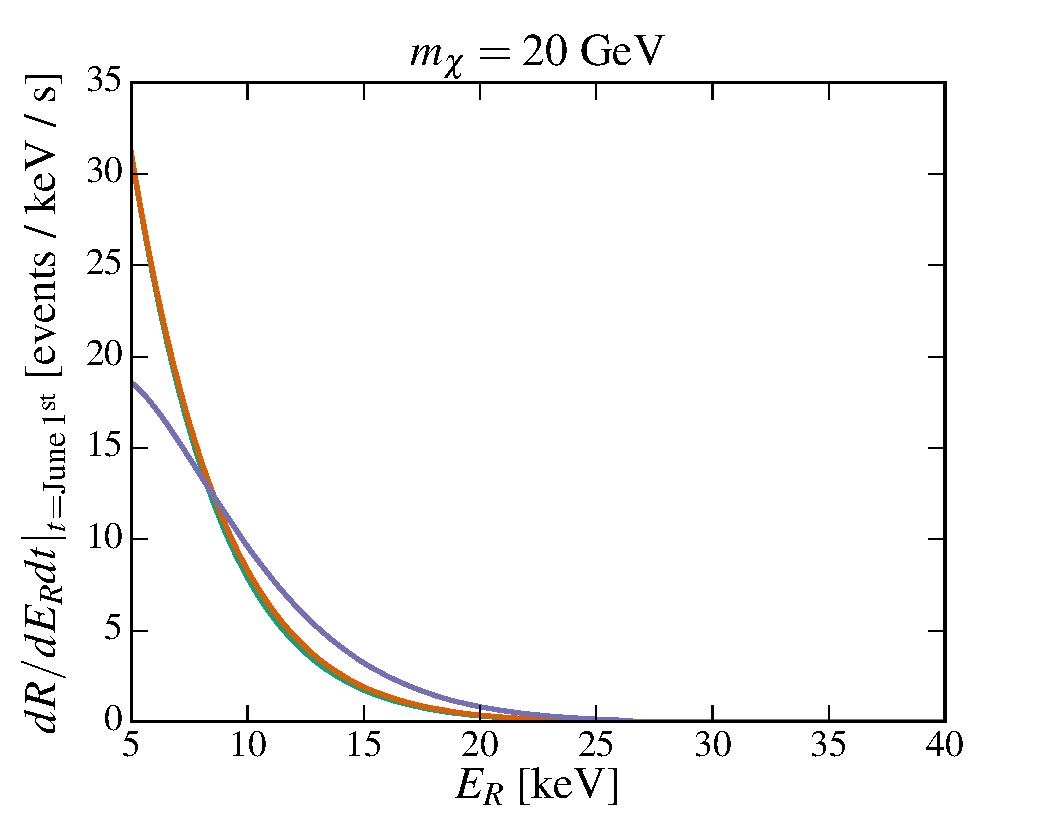
\includegraphics[width=0.49\textwidth, trim=0.cm 0.0cm 0.cm 0.0cm,clip=true]{plots/RecoilComparison_20GeV.pdf}
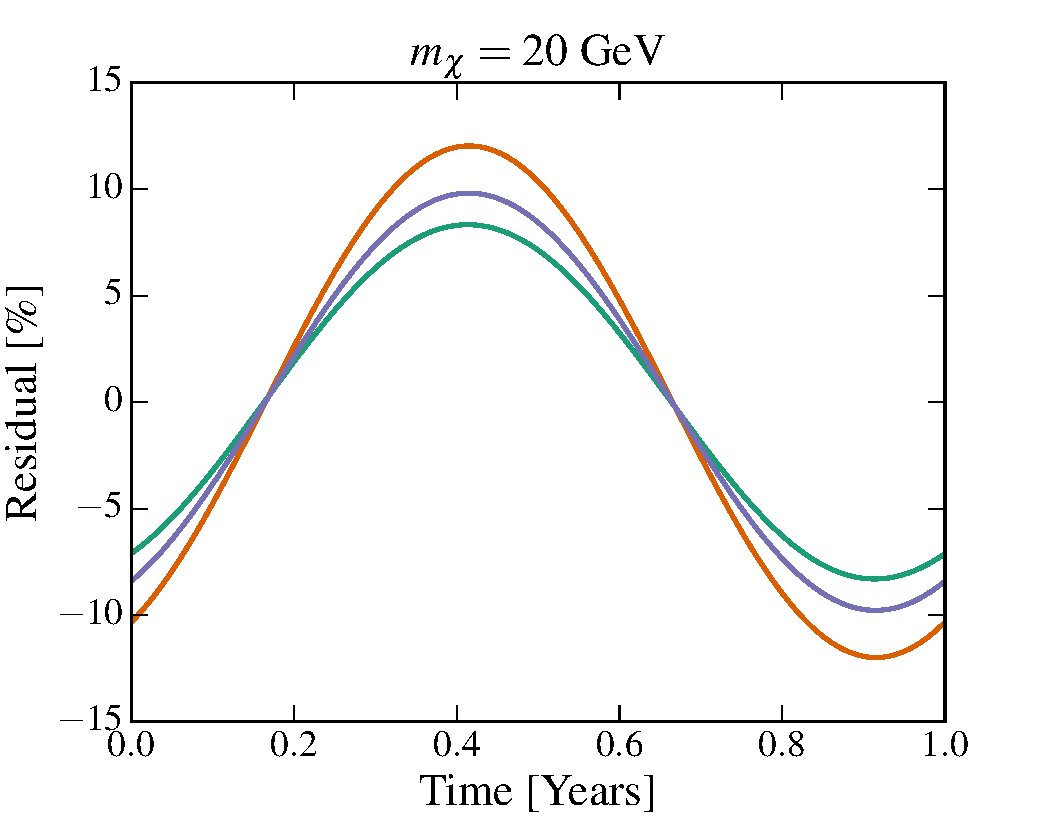
\includegraphics[width=0.49\textwidth, trim=0.cm 0.0cm 0.cm 0.0cm,clip=true]{plots/Xenon_SIvsAnapole_20GeV_Residual_Theory.pdf}
\caption{\label{fig:diff_rate_comp}
Comparison of the nuclear--recoil energy spectra (left column) and annual modulation signals (right column) between the SI (blue), anapole (black), and ED-heavy (green) interaction models on a xenon target, where the cross sections have been normalized to the current upper limits \vg{define these limits}. \emph{Left:} Differential rate evaluated at June $1^{st}$ as a function recoil energy for a $500$ GeV (top) and $20$ GeV (bottom) DM particle. \emph{Right:} Residual event rate (fractional deviation in the total event rate) as a function of time, for a $500$ GeV (top) and $20$ GeV (bottom) DM particle. }
\end{figure*}
To illustrate the effects of annual modulation as well as the previously discussed energy and velocity dependence of different interactions, \Fig{fig:diff_rate_comp} compares the energy spectra (left column) and time dependencies of the total expected event rates (right column) under several interaction scenarios: the standard SI interaction, anapole, and heavy--mediator electric dipole (ED--heavy) interaction (see \S\ref{} for a more detailed definition of the models). The panels in the top row correspond to a DM particle of $500$ GeV, and in the bottom tow $20$ GeV.  Instead of showing the differential rate as a function of time in the right--hand panels we show the residuals, defined as the fractional deviation from the time--averaged energy--integrated rate. Note, for example, that the energy spectra for the SI and ED--heavy interactions are distinct in a way that the SI and anapole interactions are not; thus, discerning the SI and anapole hypotheses using the energy spectrum alone is quite challenging, given even the most optimistic expectations for the Poisson noise \cite{Gluscevic:2015sqa}. 

However, the annual--modulation signatures of SI and anapole models can be very different, owing to a non--trivial ( $\sim | \vec v_\perp|^2$ ) velocity dependence of the cross section of the latter model. This in turn leads to different velocity integrals in \Eq{eq:dRdEr_general}, and through the effects of annual rate modulation, to different time dependence of the total event rates in the two models. For large enough DM mass, this can produce a nearly {\it opposite modulation phase} between the standard SI scenario and the anapole case! Furthermore, differential cross sections which contain multiple non--negligible terms with different velocity dependences can produce annual modulation signals entirely unique to a given target element~\cite{DelNobile:2015tza,DelNobile:2015rmp}. The expected time differences between models are however small--on the order of a few percent of the overall event rate. Nonetheless, we will show in the following that this small difference in the characteristic time dependence of the rate for different models can be used to supplement the information contained in the energy spectrum and substantially aid the process of model selection on a single target with future experiments. In the following analysis, we incorporate calculations of the annual modulation signal and the effect of gravitational focusing following the procedure of~\cite{Lee:2013wza}. 


\section{Distinguishing Scattering Models}\label{sec:procedure}

\vg{Our approach follows Gluscevic et al and consists of: pick models, simulate, analyze.... this needs expansion.}
\subsection{Summary of Models}

In order to assess the benefit from considering time dependence of the scattering signals in direct--detection analyses with future data, we focus on a subset of scattering models: a generic model of new physics, represented by a hidden $U(1)'$ that has several charged fermions $X_i$ and a heavy gauge boson $A'_\mu$ with mass $M$ that kinetically mixes with the Standard Model photon. At high energies, the Lagrangian contains
\beq \label{eq:UV-model}
\cL \supset -  m_X \bar X_i X^i + i \bar X_i \slashed D_{ij} X^j  - \frac12 M^2 A'_\mu A'^\mu  - \frac14 F'_{\mu \nu} F'^{\mu \nu} - \frac\epsilon2 F'_{\mu \nu} F^{\mu \nu}.
\eeq
At low energies, the $A'_\mu$ and most $X$ particles are integrated out. We assume a mass hierarchy that results in an electrically neutral fermion $\chi$ as the lightest degree of freedom in the dark sector. Because of the kinetic mixing, the state $\chi$ couples to the Standard Model nucleon current \cite{Gresham:2014vja},
\beq \label{eq:current}
\cJ_\mu = \partial^\alpha F_{\alpha \mu} = e \sum_{n,p} \bar N \pL Q_N \frac{K_\mu}{2m_N} -\widetilde \mu_N \frac{i \sigma_{\mu \nu}q^\nu}{2m_N} \pR N,
\eeq 
where $Q_{p(n)}=1(0)$ are the nucleon charges in units of the electron charge $e$, $K_\mu/2 = (k_\mu + k'_\mu)/2$ is the average nucleon momentum, and $\tilde{\mu}_N = {\text{magnetic moment} \over \text{nuclear magneton}}$ is the dimensionless magnetic moment of the nucleon.

The details of the masses and charges of the dark fermions $X_i$ that constitute or couple to the dark matter $\chi$ will determine the response that is measured in an experiment. We will use $\cO_\chi^\mu$ to denote the Lorentz-vector fermion bilinear that couples to the current in \Eq{eq:current}. Because we assume $\chi$ is electromagnetically neutral, the possible $\cO_\chi^\mu$ are \cite{Gresham:2014vja, Gluscevic:2015sqa}
\begin{eqnarray} \label{eq:photon-DM-ops}
\cO_{\rm \chi, Anapole}^\mu & = & g^{\rm Anapole}\bar \chi \gamma^\mu \gamma_5 \chi, \\
\cO_{\rm \chi, MD}^\mu & = & \frac{g^{\rm MD}}{\Lambda}\bar \chi i \sigma^{\mu \nu} q_\nu \chi ,\\
\cO_{\rm \chi, ED}^\mu & = & \frac{g^{\rm ED}}{\Lambda} \bar \chi i \sigma^{\mu \nu} \gamma_5 q_\nu \chi.
\end{eqnarray}
As stated above, the interaction operator for $\chi$ is determined by the dynamics of the $X$ fermion(s). The anapole current in \Eq{eq:photon-DM-ops} will arise if charged $X^\pm$ states condense to form a neutral Majorana state $\chi$ \cite{Bagnasco:1993st}. The dipole currents form if an electromagnetically neutral $X^0$ couples to an electromagnetically charged pair of partner $X^\pm$ particles (of appropriate spin) \cite{Weiner:2012gm}. The scale at which the charged $X$ states are integrated out is $\Lambda$.

The simplicity of the model in \Eq{eq:UV-model} and the rich assortment of momentum and velocity dependence that appear in the associated EFT responses illustrates how generic the ``novel responses'' are. We list the EFT classification of these operators in \Tab{tab:operators}. (This is an abbreviated version of the more exhaustive table that appeared in \cite{Gluscevic:2015sqa}, using results of \cite{Gresham:2014vja, Gluscevic:2015sqa}.
) In this work, we will focus on differentiating responses that have the same momentum scaling but different velocity dependence.
\begin{table}[tb]
\begin{centering}
\renewcommand{\arraystretch}{1.3}
\begin{tabular}{c |>{$}c<{$}| >{$}c<{$} >{$}c<{$} c } \hline
 Model name & {\rm Lagrangian} & \text{$\vec q$, $v$ Dependence} &  {\rm Response}  
\\ \hline 
 SI & \frac g{M^2}\bar \chi \chi \bar N N & 1 & M
\\ \hline 
 \multirow{2}{*}{Anapole} & \multirow{2}{*}{$\frac g{M^2}\bar{\chi} \gamma^\mu \gamma_5 \chi \, \cJ_\mu $} & v_\perp^2 & M \\  
 & & \vec{q}^2/m_N^2 & \Delta + \Sigma' 
\\ \hline
\multirow{2}{*}{\pbox{20cm}{Magnetic Dipole (Heavy)}} & \multirow{2}{*}{$\frac g{\Lambda M^2} \bar{\chi} \sigma^{\mu \nu} \chi  \, q_\nu \cJ_\mu $} & \frac{\vec q^{\,4}}{\Lambda^4}+ \frac{\vec{q}^2 v_\perp^2 }{\Lambda^2} & M \\
 & & \vec q^{\,4}/\Lambda^4 & \Delta + \Sigma' 
\\ \hline
Electric Dipole (Heavy) & \frac g{\Lambda M^2} \bar{\chi} \sigma^{\mu \nu} \gamma_5 \chi \, q_\nu \cJ_\mu  & \vec{q}^2 /\Lambda^2 & M 
\\ 
\hline 
\multirow{2}{*}{\pbox{20cm}{Magnetic Dipole (Light)}} & \multirow{2}{*}{$\frac g\Lambda \bar{\chi} \sigma^{\mu \nu} \chi F_{\mu\nu} $} & 1+ \frac{v_\perp^2 m_N^2}{\vec{q}^2 } & M \\
  & & 1 & \Delta + \Sigma' 
 \\ \hline
 Electric Dipole (Light) & \frac g\Lambda \bar{\chi} \sigma^{\mu \nu} \gamma_5 \chi F_{\mu\nu}  & m_N^2/\vec{q}^2 & M 
 \\ \hline 
\end{tabular}
\caption{Selection of operators along with their EFT dependences, adapted from \cite{Gluscevic:2015sqa}. The labels `Light' and `Heavy' in the dipole models denote the magnitude of the mediator mass relative to the characteristic momentum transfer. The nucleon electromagnetic current $\cJ_\mu$ is defined in \Eq{eq:current}; the transverse velocity $v_\perp$ and three--momentum transfer $\vec q$ are defined in terms of the collision momenta in \Eq{eq:kinematic-definitions}; and $\Lambda$ is a heavy mass or compositeness scale appearing in the dipole models. The parametric momentum and velocity dependences (third column) schematically multiply the adjacent EFT response (fourth column). }
\label{tab:operators} 
\end{centering}
\end{table}

\subsection{Simulations\label{sec:sims}}

\begin{table*}[tbp]
  \setlength{\extrarowheight}{3pt}
  \setlength{\tabcolsep}{10pt}
  \begin{center}
	\begin{tabular}{c|m{2.3cm}m{4.2cm}m{2.8cm}}  
	Label & A (Z) & Energy window [keVnr] & Exposure [kg-yr] \\
	\hline
	Xe & 131 (54) & 5-40 & 2000 \\
	Ge & 73 (32) & 0.3-100 & 100  \\
	F &  19 (9) & 3-100 & 606 \\
	\hline
	Xe(x3) & 131 (54) & 5-40 & 6000 \\
	Xe(x10) & 131 (54) & 5-40 & 20 000 \\
	XeG3 & 131 (54) & 5-40 & 40 000 \\
	\end{tabular}
  \end{center}
\caption{Mock experiments considered in this work. The efficiency and the fiducialization of the target mass are included in the exposure. The first group of experiments is chosen such to be representative of the reach of Gen2 experiments for Xe, Ge, and F. The exposure for Xe and Ge is chosen to agree with the projected exclusion curves for LZ and SuperCDMS presented in Ref.~\cite{Cushman:2013zza}. The second group of experiments is used to quantitatively assess the impact of including the timing information as a function of the exposure, i.e. the observed number of events. }
\label{tab:experiments}
\end{table*}
\begin{table*}[t] 
\setlength{\extrarowheight}{3pt}
\setlength{\tabcolsep}{12pt}
\begin{center}
\begin{tabular}{c||m{3cm}|m{3cm}|m{3cm}}
Interaction /target & Xe & Ge & F\\
\hline\hline 
$m_\chi$ [GeV] & (20, 125, 500) & (20, 125, 500) & (20, 125, 500) \\
\hline\hline 
SI& (103, 99, 98) & (9, 4, 4)& (5, 1, 2)\\ \hline
Anapole& (103, 97, 96)& (11, 5, 5)& (36, 3, 3)\\ \hline
Mag. dip. heavy& (103, 89, 87)& (3, 4, 5)& (4, 1, 1)\\ \hline
Mag. dip. light& (103, 101, 101)& (34, 14, 14)& (86, 16, 15)\\ \hline
Elec. dip. heavy& (103, 91, 88)& (4, 4, 4)& (1, 0, 0)\\ \hline
Elec. dip. light& (103, 102, 101)& (61, 15, 14)& (40, 12, 12)\\ \hline \hline
\end{tabular}
\end{center}
\caption{Predicted number of events in Gen2 experiments for various interactions with xenon, germanium, and fluorine targets assuming a DM mass of ($20$ GeV, $125$ GeV, and $500$ GeV). The predicted numbers of events are calculated using a cross section set to the current 90\% upper limits. Labels `light' and `heavy' denote the relative relation between the mediator mass and the characteristic scale of momentum transfer. }
\label{tab:pred_events}
\end{table*}
For our simulations, we consider interactions discussed in previous Section, and examine three test masses for DM particle: $20$ GeV, $125$ GeV, and $500$ GeV. In all our simulations, we optimistically set the cross section to be the value maximally allowed by LUX null results~\cite{Akerib:2016vxi} \vg{only LUX??}. Our initial analysis focuses on Gen2 experiments, specifically xenon, germanium, and fluorine based targets. Since fluorine experiments measure only the energy integrated rate, information on recoil energies of individual events are neglected in this case.  The exposure and energy window of our mock experiments are summarized in Table~\ref{tab:experiments}. Throughout the analysis we assume unit detection efficiency and zero backgrounds. In addition to the aforementioned, we also consider the potential reach of a Generation 3 (Gen3) xenon experiment, as well as various xenon experiments with exposures lying somewhere between Gen2 and Gen3 (the properties of which are summarized in Table~\ref{tab:experiments}).  The predicted number of events in these mock experiments are shown in Table~\ref{tab:pred_events}. 

For each simulation, the observed number of events is obtained by randomly selecting from a Poisson distribution with a mean given by the predicted number of events (\Eq{.}). The recoil energy and time of each event is then obtained by applying a rejection sampling algorithm to the two-dimensional differential scattering rate. \vg{citation?}

\subsection{Analysis method}

Within the Bayesian inference framework, the probability that the data $\vec{X}$ assigns to a given model $\cM_j$ is given by
\begin{equation}\label{eq:probs}
P(\cM_j) = \frac{\cE_j(\vec{X}|\cM_j)}{\sum_i \cE_i(\vec{X}|\cM_i)} \, ,
\end{equation}
where $\cE(\vec{X}|\cM)$ is the evidence of model $\cM$, defined by
\begin{equation}\label{eq:evidence}
\cE(\vec{X}|\cM) = \int d\Theta \, \cL(\vec{X}|\Theta,\cM) \, p(\Theta,\cM) \, ,
\end{equation}
and is intuitively understood to be the factor required to normalize the posterior $\cP$, \ie
\begin{equation}\label{eq:posterior}
\cP(\Theta | \vec{X}, \cM) = \frac{\cL(\vec{X}|\Theta,\cM)\, p(\Theta,\cM)}{\cE(\vec{X}|\cM)} \, . 
\end{equation}
Here, $\cL(\vec{X}|\Theta,\cM)$ is the likelihood, \ie the probability of obtaining the data, given a particular model $\cM$ and parameters $\Theta$ (for the purpose of this analysis $\Theta = \cbL m_\chi, \sigma_p \cbR$), and $p(\Theta, \cM)$ is the prior. In order to remain as agnostic as possible, we take wide priors in both $m_\chi$ and $\sigma_p$\footnote{Log priors are taken for both $m_\chi$ and $\sigma_p$, spanning $1-3000$ GeV in mass and $7$ orders of magnitude in cross section.}. In our analysis we use an unbinned extended likelihood function of the form
\begin{equation}\label{eq:likelihood}
\cL(\vec{X}|\Theta,\cM) = \frac{\mu^N}{N!} \, e^{-\mu} \, \prod_{x_i \in \vec{X}}\, \frac{1}{\mu} \, \frac{dR}{d\ER dt} \bigg|_{\ER,t \, = \, x_i} \, ,
\end{equation}
where $\mu$ is the predicted number of events, $N$ is the number of observed events, and the product runs over all the normalized differential rate evaluated at the $\ER$ and $t$ values of each observed event $x_i \equiv \cbL E_{R,i} \, , \, t_i \cbR$. When time or $\ER$ information is neglected, the differential rate is implicitly understood to be averaged over that variable. 

Our analysis proceeds as follows. We begin by simulating data for an experiment (or experiments) assuming a particular dark matter model, mass, and cross section (see Sec.~\ref{sec:sims}). We then use PyMultiNest to reconstruct the posterior defined in \Eq{eq:posterior}, and subsequently calculate the evidence for various dark matter models~\cite{pymultinest,Feroz:2008xx}\footnote{Multinest runs are performed with 2000 live points, an evidence tolerance of 0.1, and a sampling efficiency of 0.3.}. Once the evidence of various models has been computed, one can estimate the probability of successfully being able to identify the true model using \Eq{eq:probs}. This procedure is then repeated for $\simeq \cO(50)$ simulations to assess the variability in successful model identification arising from Poisson fluctuations. A model is said to be correctly identified if the probability determined using \Eq{eq:probs} is large. For the purpose of this paper, we define the boundary for successful model identification at $P \geq 90\%$. The primary quantity of interest for future direct detection experiments is then the fraction of simulations which lead to a successful model identification.    

Instead of plotting the individual probabilities of each simulation, we apply kernel density estimation (KDE) with a Gaussian kernel to determine the distribution functions of these probabilities. For of the results listed in the following section, we plot the KDE distribution for each experimental combination both with and without time, and determine the fractional success rate by integrating the distribution above the 90\% threshold. 


\section{Results}\label{sec:results}

\begin{figure}
\centering
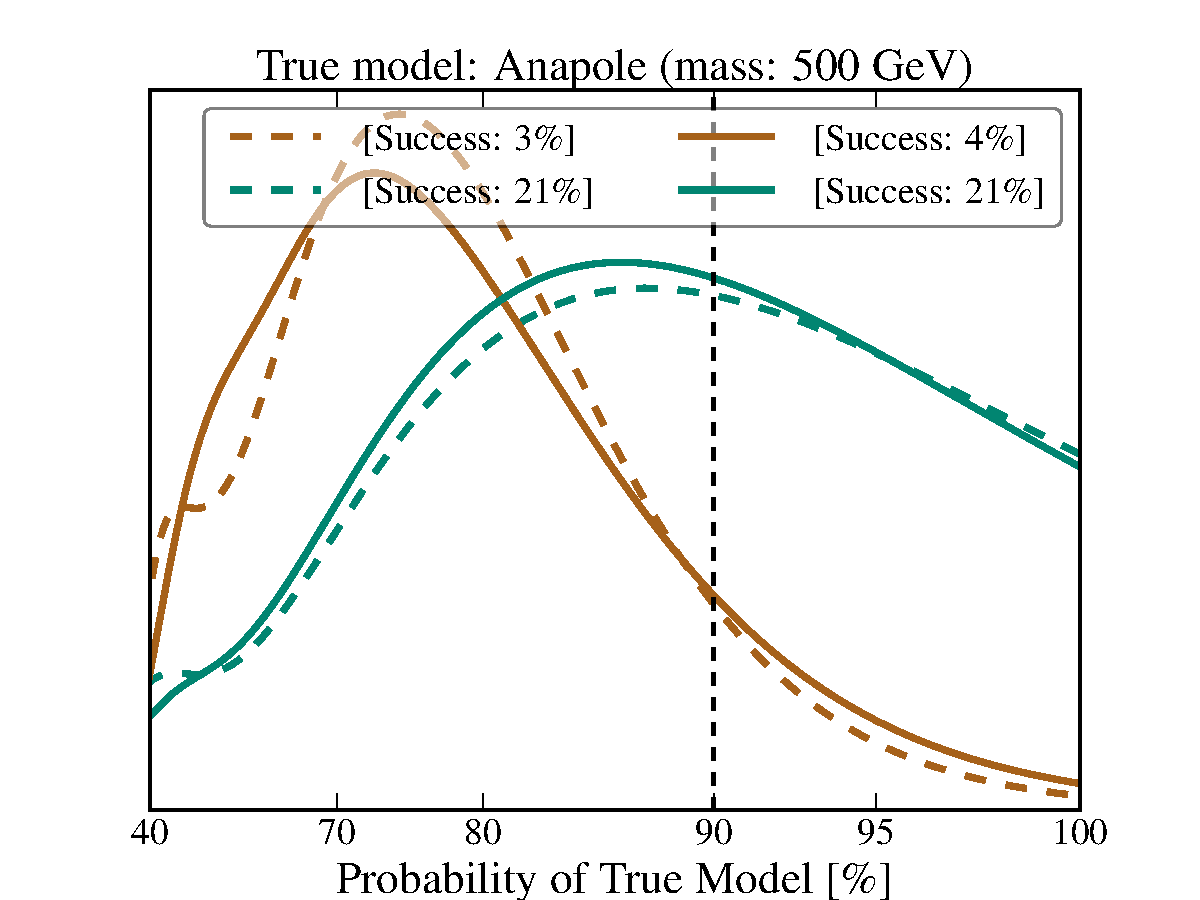
\includegraphics[width=0.45\textwidth]{plots/PDF_Single_500GeV_Anapole_50sims_Xe_vs_FGeXe_GF_TNT.pdf}
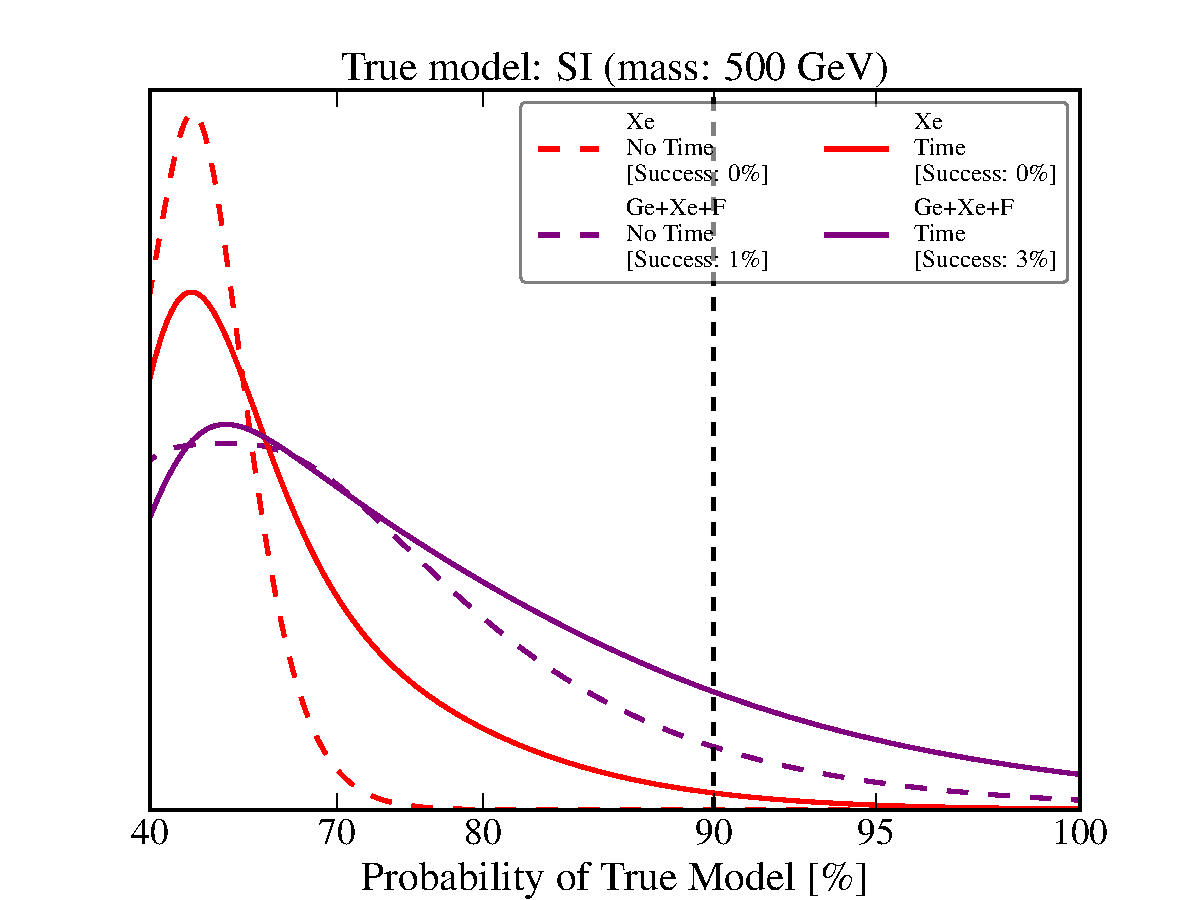
\includegraphics[width=0.45\textwidth]{plots/PDF_Single_500GeV_SI_Higgs_50sims_Xe_vs_FGeXe_GF_TNT.pdf}

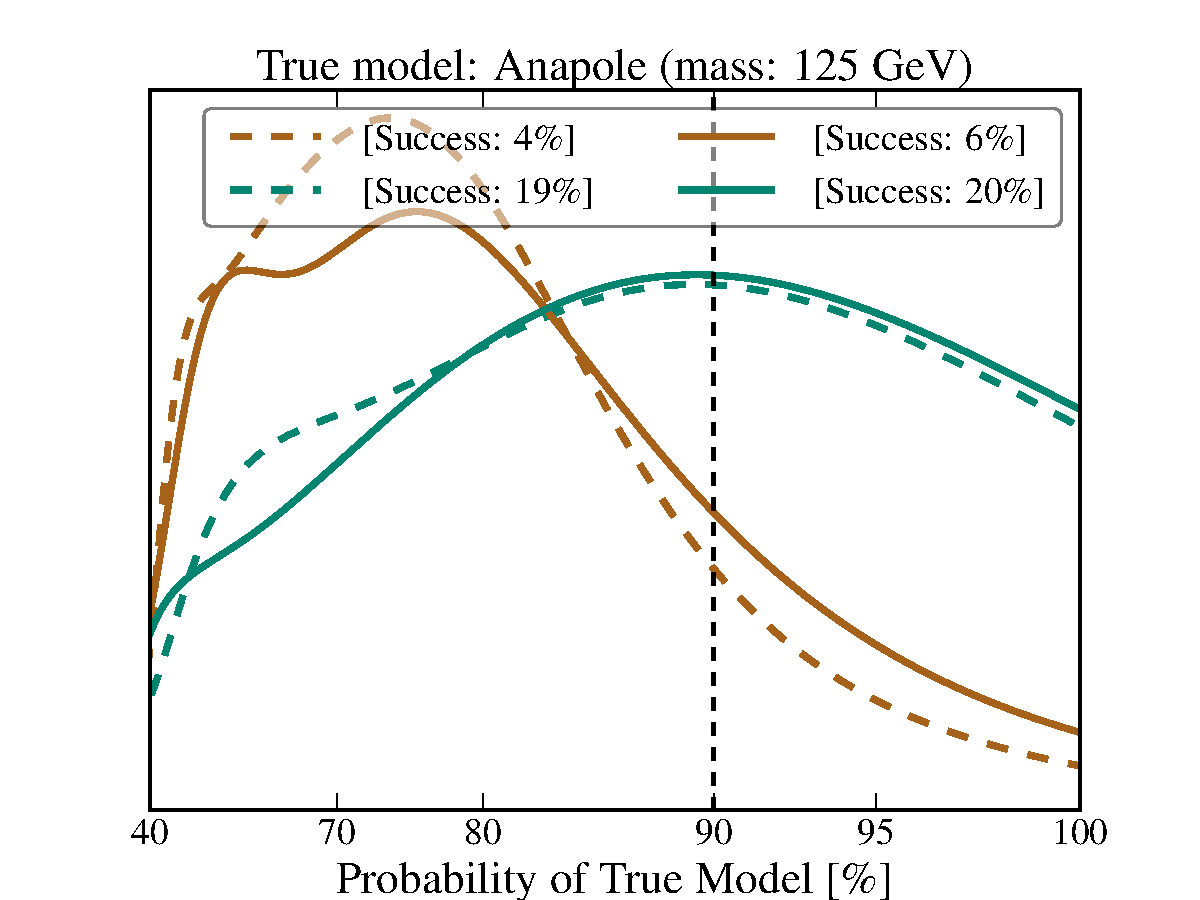
\includegraphics[width=0.45\textwidth]{plots/PDF_Single_125GeV_Anapole_50sims_Xe_vs_FGeXe_GF_TNT.pdf}
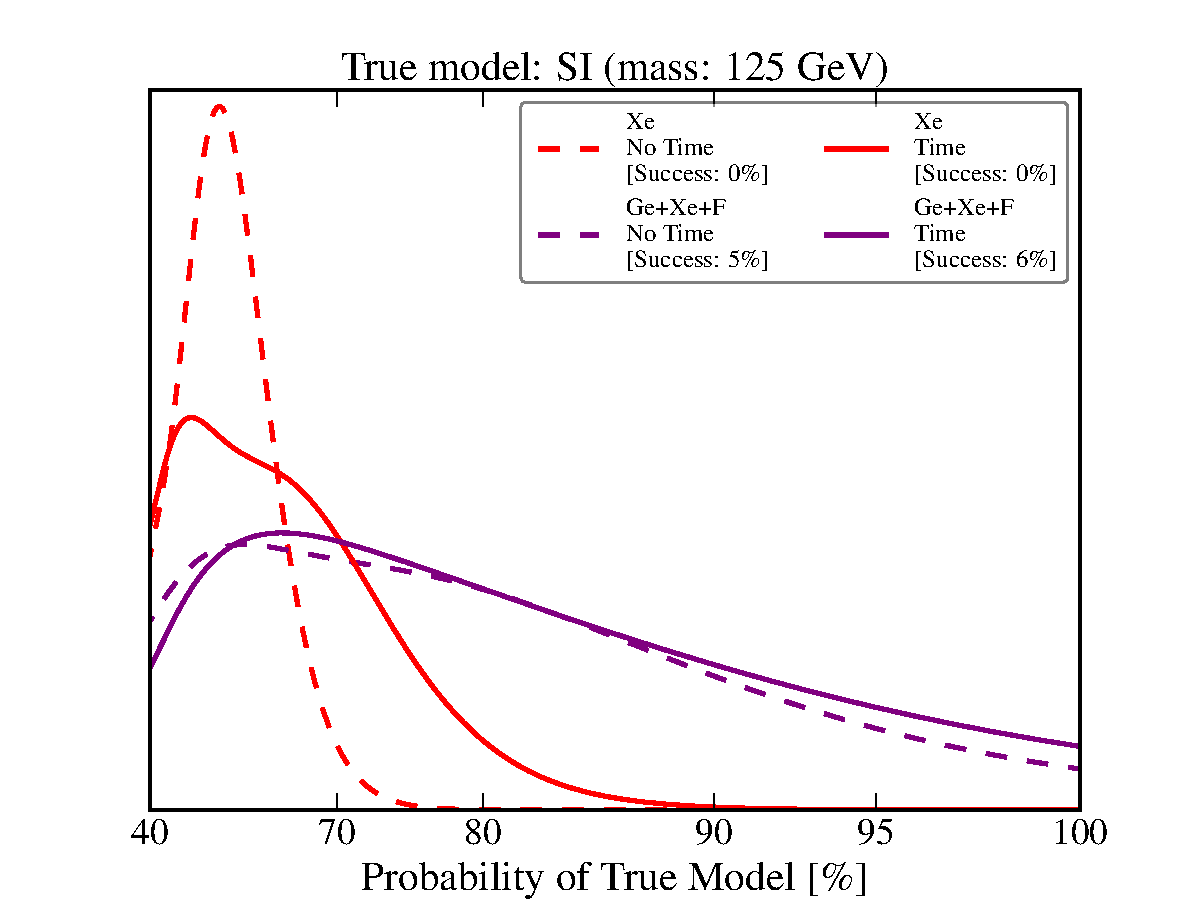
\includegraphics[width=0.45\textwidth]{plots/PDF_Single_125GeV_SI_Higgs_50sims_Xe_vs_FGeXe_GF_TNT.pdf}

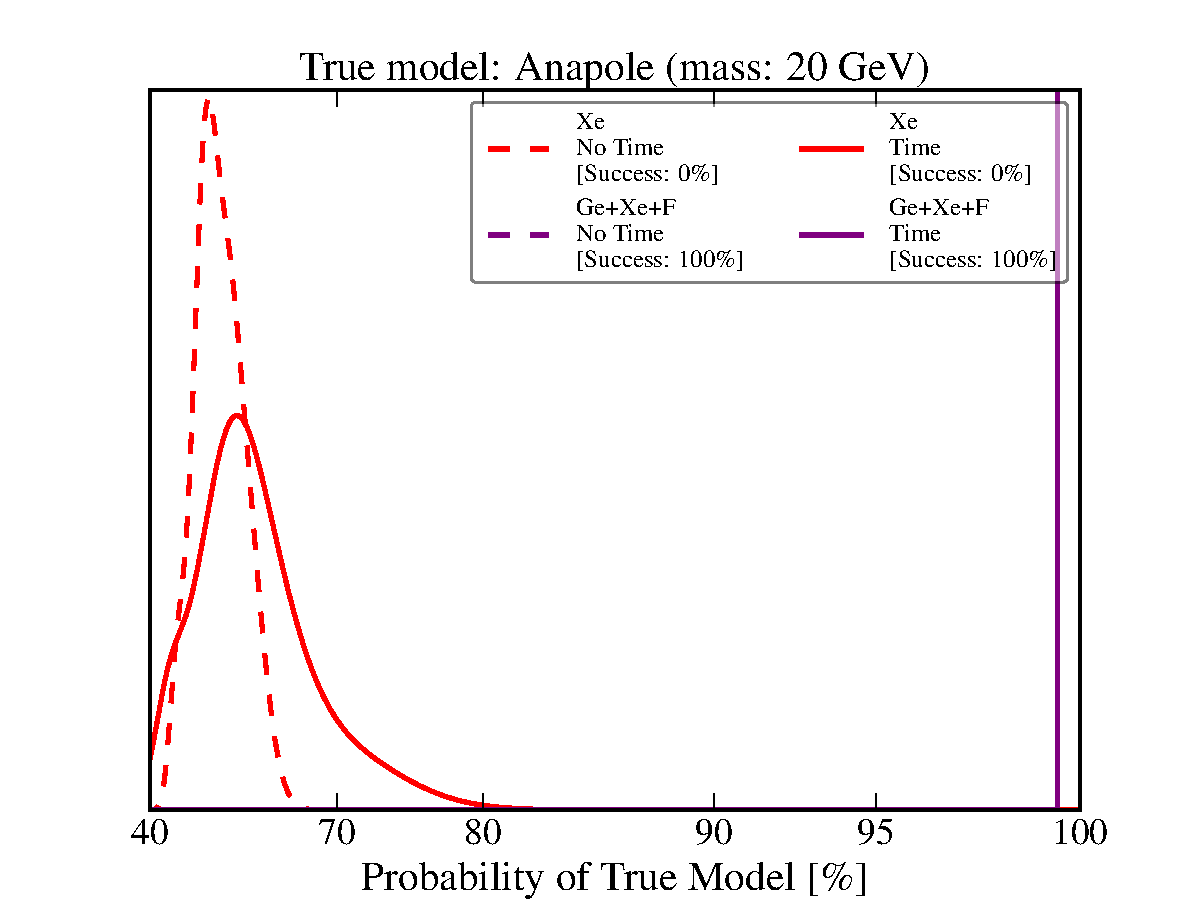
\includegraphics[width=0.45\textwidth]{plots/PDF_Single_20GeV_Anapole_50sims_Xe_vs_FGeXe_GF_TNT.pdf}
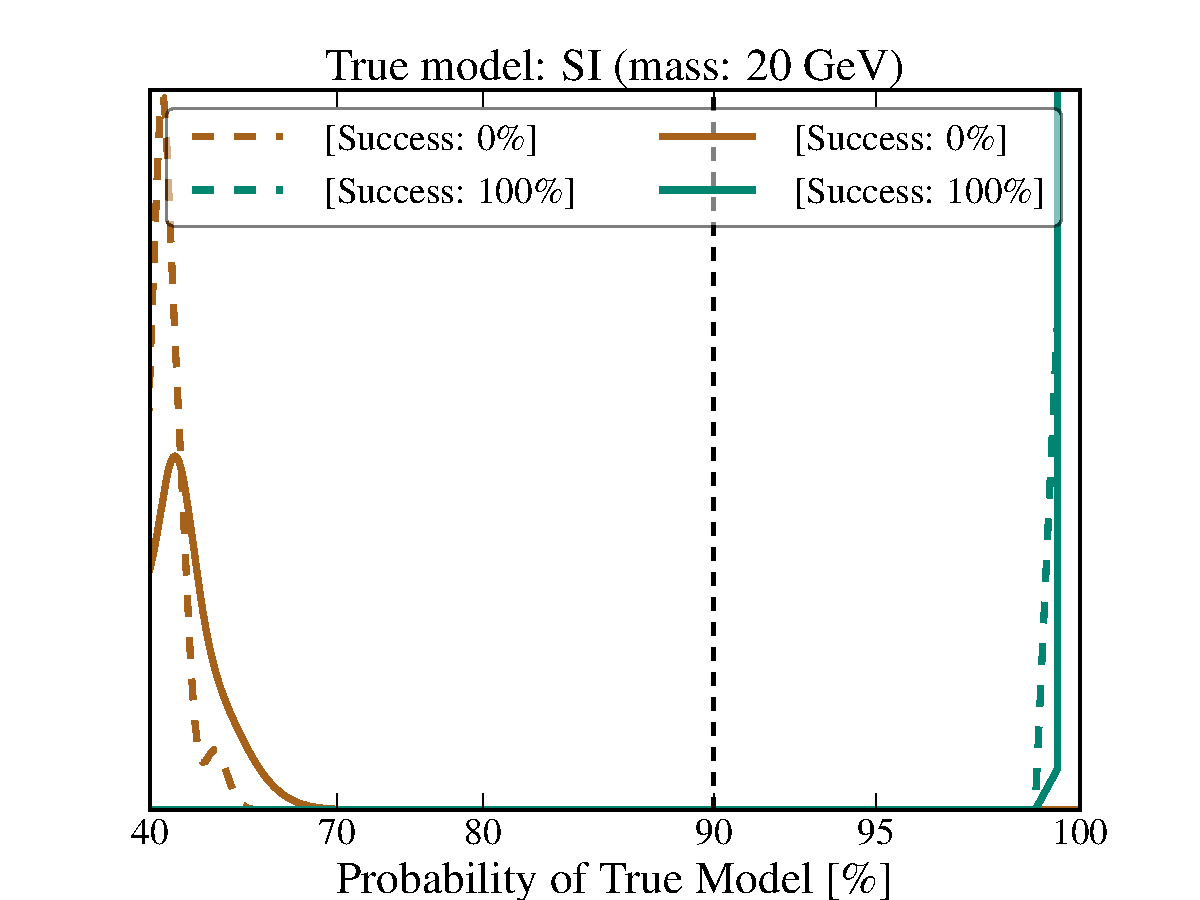
\includegraphics[width=0.45\textwidth]{plots/PDF_Single_20GeV_SI_Higgs_50sims_Xe_vs_FGeXe_GF_TNT.pdf}
\caption{\label{fig:gen2}
Model selection prospects with complimentary Gen2 targets. The reconstructed probability distribution functions for the probability of correctly identifying the right underlying interaction model are shown for the anapole (left column) and SI (right column) interactions, for a $500$ GeV (top row), $125$ GeV (middle row), and $20$ GeV (bottom row) DM particle mass. Cross sections are set to current upper limits, and the PDFs are all normalized to unity between 0 and 100$\%$. Results are shown for likelihood analyses of simulated data from a xenon experiment, and for a combined likelihood analyses of xenon, germanium, and fluorine experiments. Solid lines are the results obtained including time information for recoil events, and dashed lines are the results obtained when ignoring the modulation of the recoil rate. Success rate is defined to be the fraction of simulations for which the correct model was assigned $ \geq 90\%$ probability as compared to the wrong model.}
\end{figure}
We first examine the extent to which including time information in the analysis of Gen2 experiments can help break degeneracy between models with the same velocity dependence, using a study case of the SI and anapole interactions. Specifically, we simulate future data for the SI and anapole interactions and fit each simulation with these two models. We then compare compare Bayesian evidence of the two models to compute probability of the true underlying model (used to create a given simulation ensable), as described in \S\ref{}. We then derive the posterior probability distribution function (PDF) of the true underlying model from 50 simulations that all used the same input model with the same input parameter values.\footnote{Note that, since we only consider two compeeting models, a PDF peaked at around $50\%$ means that the data is most likely to be agnostic between the two models--they both are most likely to provide comparably good fits, and this is the most pessimistic outcome possible. A tail of the distribution at high true--model probabilities, or a PDF shift in that direction is an improvement over that case.} \Fig{fig:gen2} shows the results of this exercise for the anapole (left column) and SI (right column) interactions, for likelihood analysis only for xenon simulations, or for a joint likelihood analysis performed on a combination of data obtained on xenon, germanium, and fluorine experiments. Test DM particle masses used for the simulations are: $500$ GeV (top panels), $125$ GeV (middle panels), and $20$ GeV (bottom panels), and the input cross sections are always set to their respective current upper limits. We show the results obtained both without taking into account time dependence of the signals (dashed lines), and including (solid lines) the modulation analysis. 

Consistent with the results of~\cite{Gluscevic:2015sqa}, we find that the two models can be confidently distinguished for a signal close to the current detection threshold, provided Gen2--level exposure on xenon and a detection with a fluorine experiment, but only if data from these experiments are jointly analyzed (xenon and germanium experiments are not complementary in the same sense and their combination does not significantly improve prospects for model selection, and thus we do not display results for this case). For a low--mass DM particle (20 GeV), the improvement upon combining these two types of experiment is drastic: the PDF of possible model--selection outcomes entirely shifts to a delta--function at 100$\%$ probability in favor of the right model. For intermediate and high masses, the prospects are still visibly improved, but not very optimistic (at best on the level of $\sim$20$\%$ success rate), mostly due to the reduced scattering rate on fluorine.  

\begin{figure*}
\centering
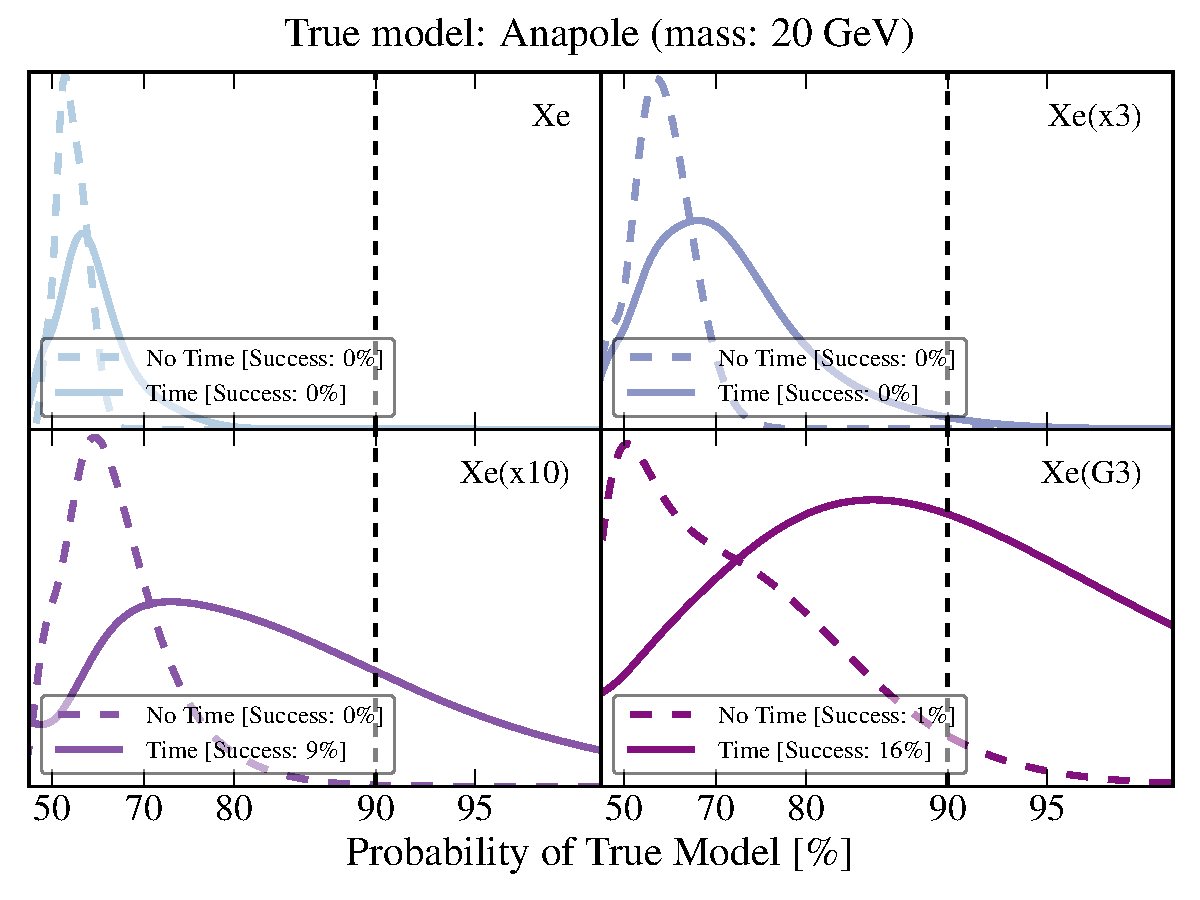
\includegraphics[width=0.7\textwidth]{plots/PDF_20GeV_Anapole_50sims_Xe_Xe3x_Xe10x_XeG3_GF_TNT.pdf}
\caption{\label{fig:20gev_anapole_XeFull_TNT_GF}
Model selection prospects for a single target (xenon), including (solid lines) and neglecting (dashed lines) time information in likelihood analysis. The normalized probability distribution functions are plotted for the posterior probability of the right underlying model--the anapole interaction of a 20 GeV DM particle. Panels from left to right, top to bottom, correspond to experimental exposures of 2, 6, 20, and 40 ton--years, respectively. Simulations used to obtaine these results all use input cross sections at their current upper limit. Percent chance for successful model identification (defined here as having $\geq 90 \%$ probability assigned to the anapole model) is provided in the legend.}
\end{figure*}
\begin{figure*}
\centering
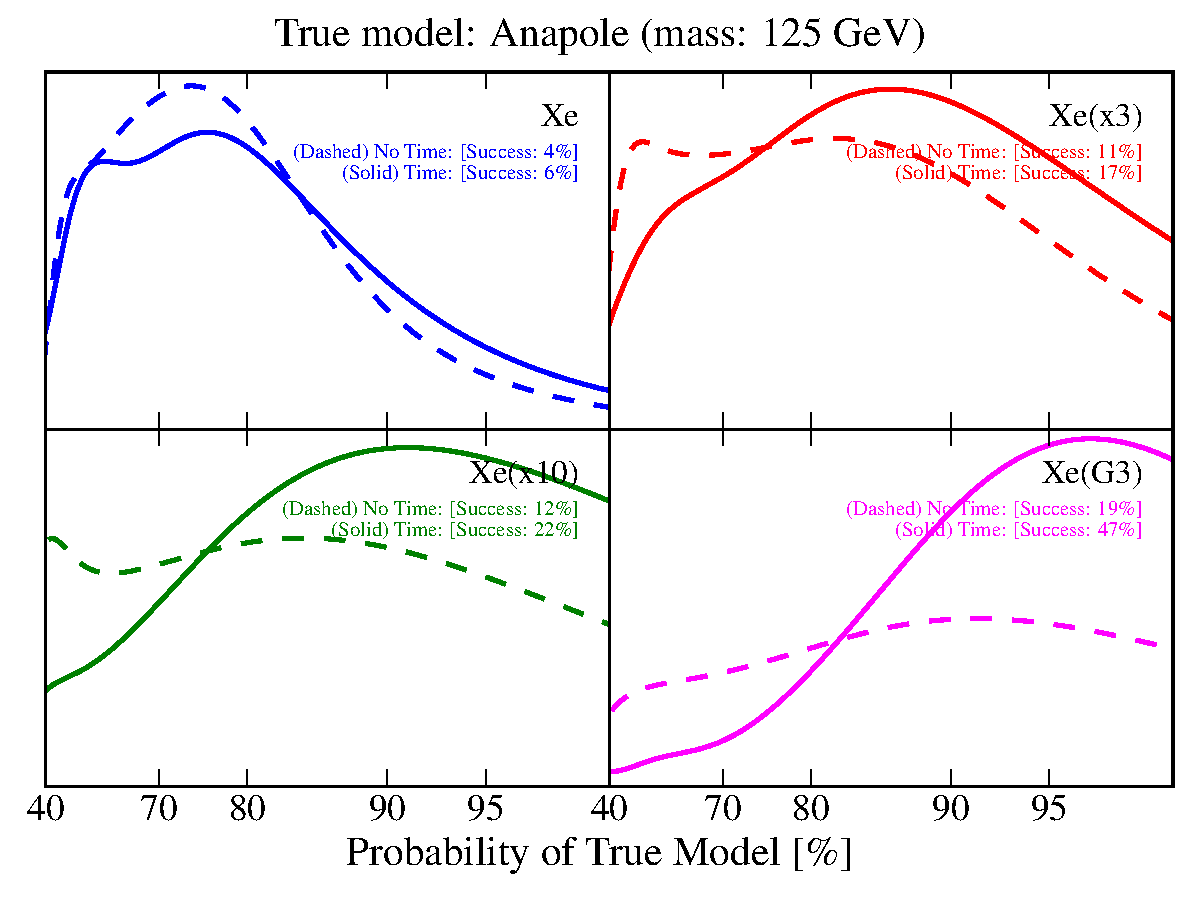
\includegraphics[width=0.7\textwidth]{plots/PDF_125GeV_Anapole_50sims_Xe_Xe3x_Xe10x_XeG3_GF_TNT.pdf}
\caption{\label{fig:125gev_anapole_XeFull_TNT_GF}
Same as Fig.~\ref{fig:20gev_anapole_XeFull_TNT_GF} but for $125$ GeV dark matter.}
\end{figure*}
\begin{figure*}
\centering
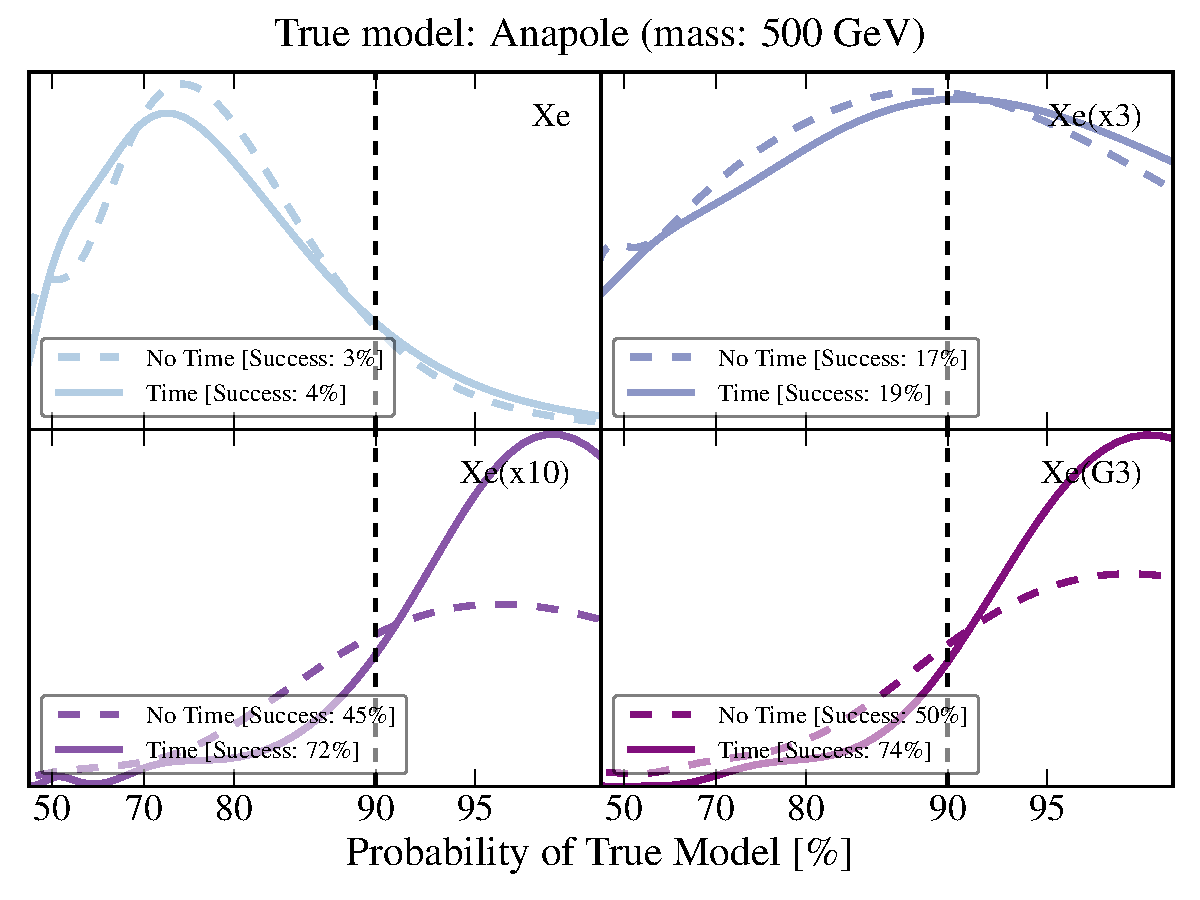
\includegraphics[width=0.7\textwidth]{plots/PDF_500GeV_Anapole_50sims_Xe_Xe3x_Xe10x_XeG3_GF_TNT.pdf}
\caption{\label{fig:500gev_anapole_XeFull_TNT_GF}
Same as Fig.~\ref{fig:20gev_anapole_XeFull_TNT_GF} but for $500$ GeV dark matter.}
\end{figure*}
\begin{figure*}
\centering
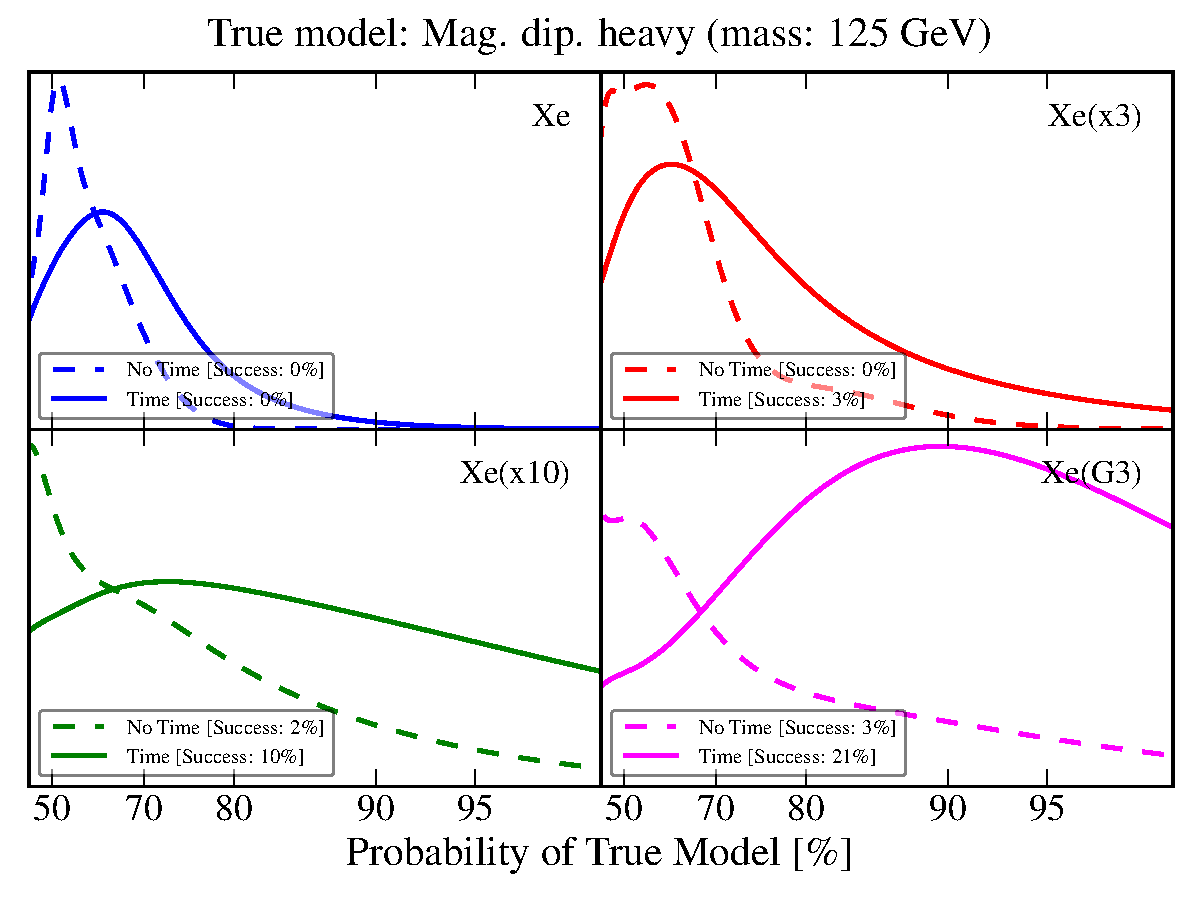
\includegraphics[width=0.7\textwidth]{plots/PDF_125GeV_Magdipheavy_50sims_Xe_Xe3x_Xe10x_XeG3_GF_TNT.pdf}
\caption{\label{fig:125gev_Mag.dip.heavy_XeFull_TNT_GF}
Same as Fig.~\ref{fig:20gev_anapole_XeFull_TNT_GF}, but now assessing the ability of xenon experiments to break the degeneracy of the magnetic dipole (heavy mediator) and electric dipole (heavy mediator) interactions, instead of SI and anapole interactions. Simulations assume a $125$ GeV DM particle and and a magnetic--dipole interaction.}
\end{figure*}
\begin{figure*}
\centering
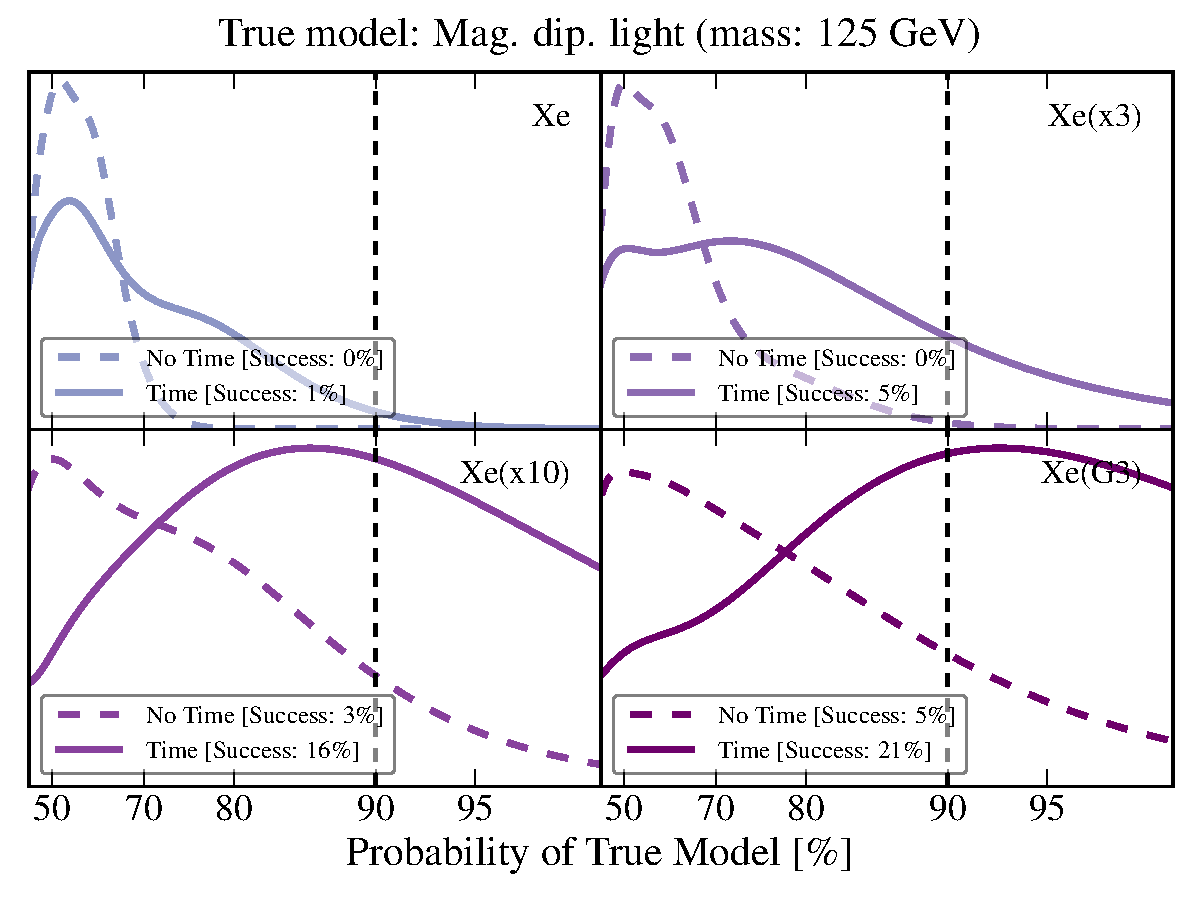
\includegraphics[width=0.7\textwidth]{plots/PDF_125GeV_Magdiplight_50sims_Xe_Xe3x_Xe10x_XeG3_GF_TNT.pdf}
\caption{\label{fig:125gev_Mag.dip.light_XeFull_TNT_GF}
Same as \Fig{fig:125gev_Mag.dip.heavy_XeFull_TNT_GF} but for a light mediator case. }
\end{figure*}
On the other hand, comparison of PDF displayed in solid and dashed lines demostrates that inclusion of time information only negligibly changes model--selection prospects for Gen2 level of exposures. Given that Gen2 experiments will optimistically detect on the order of $\simeq 100$ events, the statistical sample will be insufficient to clearly detect differences in the modulation signal that would otherwise aid differentiation between the two interactions. It is thus not surprising that analyzing Gen2 data with time has a minimal effect on model selection (see \eg Sec.~4 of \cite{DelNobile:2015nua} for an estimation of the number of events needed for phase measurement).

The question than arises of how many events are needed before the inclusion of time information can significantly help model selection prospects--and we address it in the context of xenon--based experiments in Figs.~\ref{fig:20gev_anapole_XeFull_TNT_GF}--\ref{fig:500gev_anapole_XeFull_TNT_GF}. In this Figure, we show the prospects (PDF of possible analysis outcomes) of successful model selection, given different exposures in the same experiment: a 2, 6, 20, and 40 ton--year. Simulations used for this Figure are all assuming anapole interaction (the results for the SI interaction are qualitatively similar and we defer the SI analogues of these Figures to Appendix A), and a DM mass of 20, 125, and 500 GeV DM particle mass, respectively. We show results for likelihood analyses that neglect to account for the time dependence (dashed lines), and for those that include it (solid lines). 

From these Figures, we see that the addition of time information drastically improves prospects for successful model selection in case of light DM particle (the solid--line PDFs are substantially shifted to the right in \Fig{fig:20gev_anapole_XeFull_TNT_GF}). But in spite of this, even with a Gen3 xenon experiment, there is only about $\simeq 16\%$ chance that data will be able to tell apart these two interactions with confidence. \Fig{fig:diff_rate_comp} gives an intuition for interpreting this outcome: not only are the recoil spectra from the SI and anapole interactions (measured with a xenon experiment) more degenerate for light than for heavy DM particles, but the modulation phase follows the same trend in mass (for conventional velocity dependent cross sections, see ~\cite{DelNobile:2015tza,DelNobile:2015rmp}); thus, even when including time information into the analysis, a single target still requires large even number counts in order to successfully enable model selection between these models.

At larger DM particle masses, however, the recoil energy spectra are less degenerate, allowing for better model discrimination at fixed exposure. This is, in part, because a heavier DM particle allows probing regions of parameter space where the anapole and SI interaction are out of phase (see again \Fig{fig:diff_rate_comp}). Figs.~\ref{fig:125gev_anapole_XeFull_TNT_GF} and \ref{fig:500gev_anapole_XeFull_TNT_GF} indeed confirm that heavier DM candidates allow for better model discrimination of these models, particularly when time is included in the analysis. From these Figures, we see that including time in the analysis can improve model selection in Gen3 experiments by as much as $\simeq 30\%$ for heavy DM, where the phases of the modulation signal for these two interactions may be misaligned by as much as $\simeq 5$ months. Finally, it is important to keep in mind that all the results displayed in these Figures assume the most optimistic number of observed recoil events. In light of this, in spite the improvement obrained through inclusion of time information in the analysis demonstrated in these Figures, it is likely that model selection with Gen3 experiments will still be challenging using a single target; most likely, the experiments will need to exploit target complimentarily and perform joint likelihood analyses in order to fully break the SI--anapole type of degeneracy and ensure the highest chance of correctly identifying the interaction at hand. 

The goal of this work was primarily a quantitative assessment of whether time information can be exploited in future direct--detection analyses to break degeneracies in the recoil spectra of different interaction models---and SI and anapole interactions provided a particularly illuminating study case for this purpose. However, the main conclusions presented in this Section hold for other sets of interaction models as well, and we now briefly illustrate this point. In \Figs{fig:125gev_Mag.dip.heavy_XeFull_TNT_GF}{fig:125gev_Mag.dip.light_XeFull_TNT_GF} we consider a comparison of the magnetic dipole and electric dipole interactions for a $125$ GeV DM particle, assuming a heavy (\Fig{fig:125gev_Mag.dip.heavy_XeFull_TNT_GF}) and light (\Fig{fig:125gev_Mag.dip.light_XeFull_TNT_GF}) mediator. As before, we consider putative detections in future xenon experiments with exposures varying from 2 to 40 ton--years. The results are rather similar to the SI and anapole comparison in that Gen3 experiments can expect a $\simeq 20\%$ improvement in model selection when time is included in the analysis, but again necessitate target complementarity to have a high chance of confidently differentiating between these interactions.

%%%%%%%%%%%%%%%%%%
\section{Summary and Discussion}\label{sec:conclusion}
We have considered here the potential impact of using time information in the likelihood analysis of data from future direct detection experiments in order to break degeneracies between the recoil energy spectra of different DM--baryon interaction models. Specifically, we performed a statistical assessment of the prospects for successful Bayesian model selection between different interaction models, using an ensamble of simulations that account for the impact of Poisson fluctuations on possible analysis outcomes. 

As a study case, we used comparison betwee the standard spin--independent interaction and anapole dark matter, but also demonstrated that the main findings hold for other degenerate interaction models as well. We explored three different test dark--matter masses, and focused specifically on the most optimistic case where the cross sections for all interactions saturate current upper limits. 

We found that even under the most optimistic of circumstances, including time information in the analysis of Gen2 direct detection does not significantly improve prospects for successul interaction--model selection. Rather, correct model identification in Gen2 experiments will almost certainly require measurements and combined analyses on multiple target elements. We found that for the inclusion of time information to significantly increase chances for successul model selection (by $\simeq \cO(10)\%$), given a single target element, $\simeq \cO(1000)$ events must be observed for a 20 GeV, and $\cO(300)$ for a 500 GeV dark matter particle. \vg{check previous statement. lets also discuss this mode on skype. also, is this consistent finding with previous-work oom guesses? if so, we should say it.} Furthermore, even if time is exploited in Gen3 xenon experiments, target complementarity must also be exploited to unequivocally differentiate between different models. \vg{a few words of discussion should be added here to mention that this is esp true if the signal is NOT as large as possible, and what happens in that case.}

In the event of a putative signal, direct detection experiments will be charged with the difficult task of illuminating the high energy behavior of dark matter solely from the observed low--energy recoils. This is a particularly daunting task in light of the fact that many feasible dark matter models produce nearly degenerate recoil spectra. Exploiting all of the information available, including the time information of nuclear recoils in a manner demonstrated in the analyses we employ in this work, will be necessary to make definitive statements regarding the true particle nature of dark matter.

\bigskip

\textbf{Acknowledgments.} SW is supported under the University Research Association (URA) Visiting Scholars Award Program, and by a UCLA Dissertation Year Fellowship. VG gratefully acknowledges the support of the Schmidt Fellowship at the Institute of Advanced Study. %Fermilab is operated by Fermi Research Alliance, LLC, under Contract No. DE-AC02-07CH11359 with the US Department of Energy. 

\appendix

\section{Model Selection Prospects in Xenon (SI Interaction)}
We present in Figs.~\ref{fig:20gev_SI_Higgs_XeFull_TNT_GF}--\ref{fig:500gev_SI_Higgs_XeFull_TNT_GF} the model selection prospects for various exposures on a xenon experiment, including (solid lines) and neglecting (dashed lines) information on the modulation of the recoil rate, and assuming the SI interaction is the true model. Results are shown for $20$ GeV (\Fig{fig:20gev_SI_Higgs_XeFull_TNT_GF}), $125$ GeV (\Fig{fig:125gev_SI_Higgs_XeFull_TNT_GF}), and $500$ GeV (\Fig{fig:500gev_SI_Higgs_XeFull_TNT_GF}) DM particle. Results are similar to those presented in \Sec{sec:results} for the case of the anapole interaction. 


\begin{figure*}
\centering
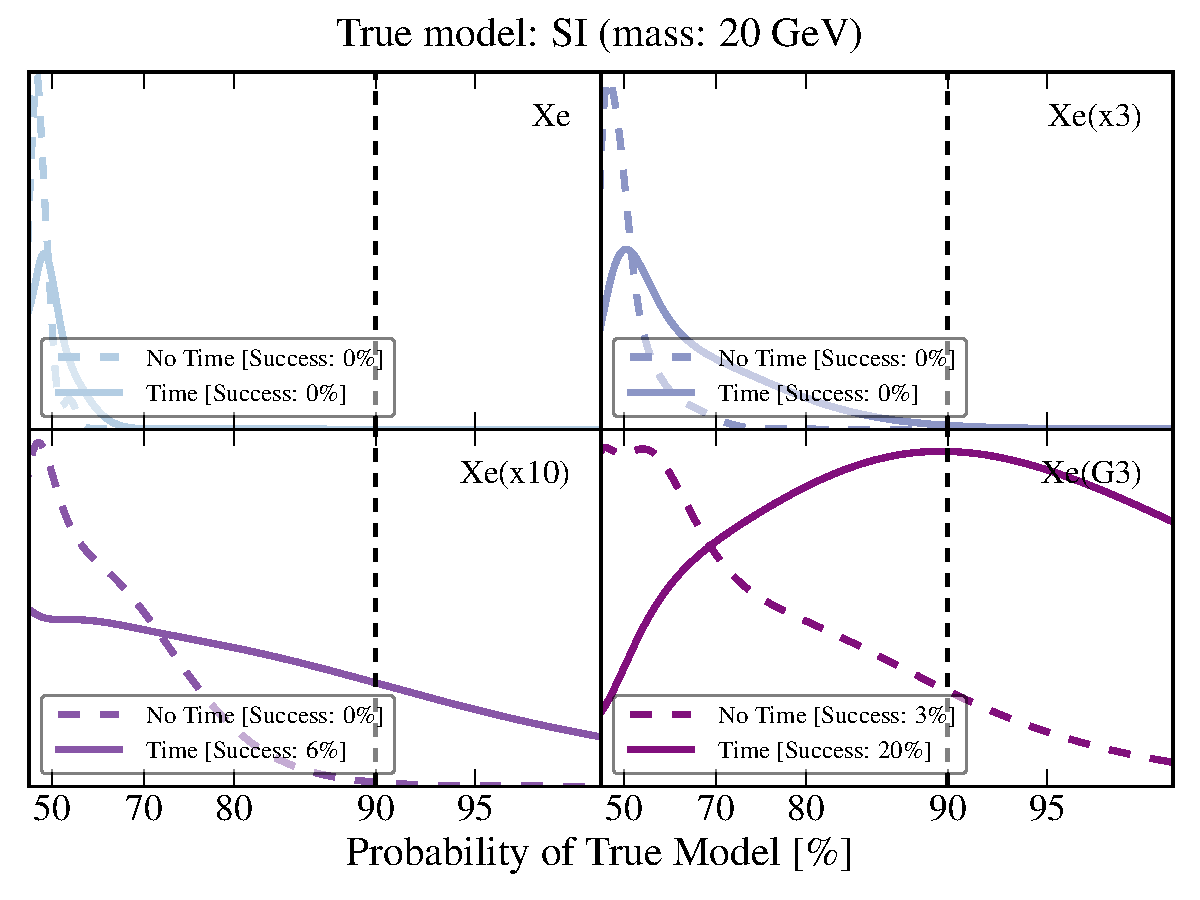
\includegraphics[width=0.7\textwidth]{plots/PDF_20GeV_SI_Higgs_50sims_Xe_Xe3x_Xe10x_XeG3_GF_TNT.pdf}
\caption{\label{fig:20gev_SI_Higgs_XeFull_TNT_GF}
Same as Fig.~\ref{fig:20gev_anapole_XeFull_TNT_GF} but for the SI interaction as the true model.}
\end{figure*}


\begin{figure*}
\centering
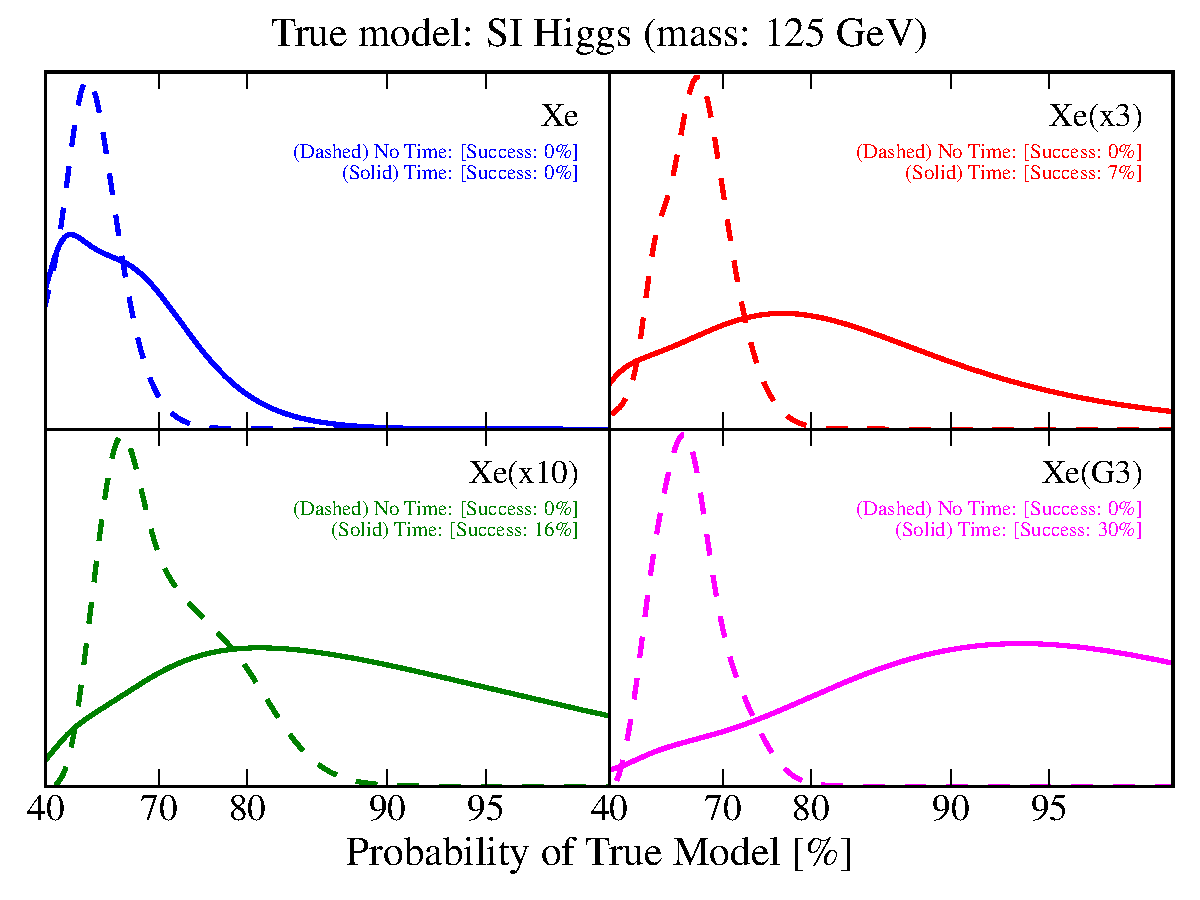
\includegraphics[width=0.7\textwidth]{plots/PDF_125GeV_SI_Higgs_50sims_Xe_Xe3x_Xe10x_XeG3_GF_TNT.pdf}
\caption{\label{fig:125gev_SI_Higgs_XeFull_TNT_GF}
Same as Fig.~\ref{fig:20gev_anapole_XeFull_TNT_GF} but for a $125$ GeV DM and the SI interaction as the true model.}
\end{figure*}


\begin{figure*}
\centering
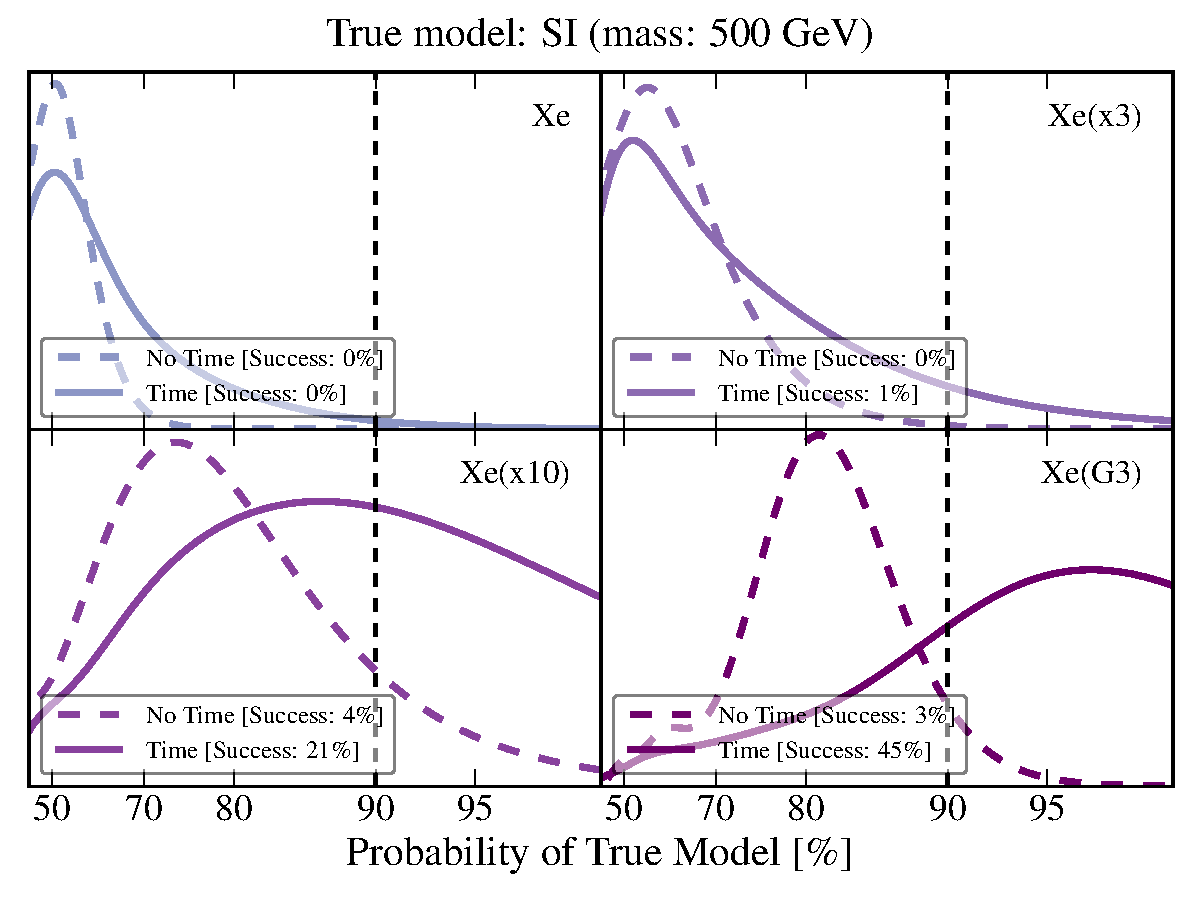
\includegraphics[width=0.7\textwidth]{plots/PDF_500GeV_SI_Higgs_50sims_Xe_Xe3x_Xe10x_XeG3_GF_TNT.pdf}
\caption{\label{fig:500gev_SI_Higgs_XeFull_TNT_GF}
Same as Fig.~\ref{fig:20gev_anapole_XeFull_TNT_GF} but for a $500$ GeV DM and the SI interaction as the true model.}
\end{figure*}

\bibliographystyle{JHEP}
\bibliography{mod-sel}

\end{document}